\documentclass[12pt,oneside]{uhthesis}
\usepackage{subfigure}
\usepackage[ruled,lined,linesnumbered,titlenumbered,algochapter,english]{algorithm2e}
\usepackage{amsmath}
\usepackage{amssymb}
\usepackage{amsbsy}
\usepackage{caption,booktabs}
\usepackage{url}
\usepackage{graphicx}
\captionsetup{
	justification = centering
}
%\usepackage{mathpazo}
\usepackage{float}
\usepackage{todonotes}
\floatstyle{plaintop}
\restylefloat{table}

\renewcommand{\tablename}{Tabla}
\renewcommand{\listalgorithmcfname}{Índice de Algoritmos}%
%\dontprintsemicolon
\SetAlgoNoEnd


\title{Implementaci\'on de la recuperaci\'on de imágenes usando una ordenación suave de sus parches}
\author{Daniel Alberto Garc\'ia P\'erez}
\advisor{ Dra. Marta Lourdes Baguer}
\degree{Licenciado en Ciencia de la Computaci\'on}
\faculty{Facultad de Matemática y Computación}
\date{5 de octubre del 2021}
\logo{Graphics/uhlogo}
\makenomenclature


\newcommand{\II}{\textit{image inpainting}}
\newcommand{\z}{\mathbf{z}}
\newcommand{\Z}{\mathbf{Z}}
\newcommand{\y}{\mathbf{y}}
\newcommand{\Y}{\mathbf{Y}}
\newcommand{\x}{\mathbf{x}}
\newcommand{\X}{\mathbf{X}}
\renewcommand{\P}{\mathbf{P}}
\renewcommand{\H}{\mathit{H}}
\newcommand{\B}{\mathbf{B}}
\newcommand{\yhat}{\hat{\mathbf{y}}}
\newcommand{\Yhat}{\hat{\mathbf{Y}}}
\newcommand{\ztilde}{\tilde{\mathbf{z}}}
\newcommand{\Ztilde}{\tilde{\mathbf{Z}}}
\newcommand{\yhattilde}{\hat{\tilde{\mathbf{y}}}}
\newcommand{\Yhattilde}{\hat{\tilde{\mathbf{Y}}}}
\newcommand{\TSP}{\textbf{TSP}}

\begin{document}

\frontmatter
\maketitle

%\begin{dedication}

[Redactar dedicatoria]

\end{dedication}
\begin{acknowledgements}

  Gracias a las personas que me apoyaron a lo largo del proceso de investigación y escritura de esta tesis. 
  [Redactar esto]
\end{acknowledgements}
\begin{opinion}
Opinion de la profe Marta
[Redactar esto] 

\end{opinion}
\begin{abstract}
	[Redactar el abstract]  
\end{abstract}
\newpage

\begin{center}
	{\large \textbf{Objetivos de la tesis}}
\end{center}
\qquad 

\qquad\textbf{Objetivo general de la tesis}: Restaurar im\'agenes mediante un esquema basado en la ordenaci\'on suave de los parches.

\qquad 

\qquad 

\qquad\textbf{Objetivos espec\'{\i}ficos de la tesis}:
\begin{enumerate}
	\item Estudio del esquema de restauraci\'on basado en el algoritmo de ordenamiento suave de los parches de una imagen.
	\item Implementaci\'on del algoritmo y del esquema en general.
	\item Exprimentar con dos casos de estudio. Uno donde se conoce la imagen real y otro donde no.
	\item Comparar los resultados del experimento con otros algoritmos del estado del arte.
\end{enumerate}
\tableofcontents
\listoffigures
\listoftables
\listofalgorithms

\mainmatter

\begin{introduction}\label{chapter:introduction}

Los primeros pasos en la recuperaci\'on de imágenes con un enfoque científico datan de antes del siglo \textbf{XVIII}. Pietro Edwards \cite{itwiki:PE}, quien dirigía la restauraci\'on de las pinturas p\'ublicas de Venecia, Italia, ten\'ia la intenci\'on de restaurar las obras de arte que atesoraba su ciudad lo m\'as fiel posible a su respectivo autor original. Las obras de arte plasmadas sobre un lienzo, un mural o en el techo de una catedral inevitablemente sufren el paso del tiempo. A lo largo de los años se agrietan, pierden poco a poco el color o incluso pueden desprenderse algunas de sus partes. Es trabajo de un grupo de especialistas restaurar las mismas para que estas persistan a lo largo de la historia en un estado lo m\'as similar posible al resultado inmediato de su autor. Uno de los ejemplos m\'as famosos es el mural pintado por Leonardo Da Vinci: \textit{La \'ultima cena} \cite{wiki:CR-TLS}. Esta obra ha pasado varios ciclos de conservaci\'on-restauraci\'on en manos de diferentes personas, lo que ha llevado a que hoy en d\'ia se encuentre en un estado muy delicado. El uso de los avances tecnológicos logr\'o frenar su continuo deterioro pero existen medidas muy estrictas para su exhibición al p\'ublico. Algo similar ocurre con las fotos que nos legaron nuestros abuelos y padres, en no pocas ocasiones se dañan al ser dobladas o por su exposici\'on a la humedad, y se deben someter a un proceso cuidadoso de restauraci\'on. Hoy en d\'ia con la llegada de la era digital y el establecimiento del Internet, las fotos que le dejaremos a nuestros hijos ser\'an en su mayor\'ia digitales. Las im\'agenes digitales no se deterioran físicamente, el \'unico daño al que est\'an expuestas es a su posible eliminaci\'on o a que se corrompa el archivo digital, lo cual no constituye una amenaza pues al ser subidas al Internet se crean suficientes copias de seguridad para evitar su p\'erdida. Por ende todos nuestros recuerdos, obras de artes, y todo tipo de datos se encuentran a salvo de forma digital en Internet y se conservar\'an en su estado original para la eternidad.

Usualmente para almacenar una imagen digital en la memoria se representa en forma de matriz. Esta representaci\'on tan conveniente ha permitido la aplicaci\'on de resultados matem\'aticos y de la computaci\'on que mejoran considerablemente la calidad de la imagen. Con las nuevas tecnolog\'ias surgen nuevas y \'utiles aplicaciones de la restauraci\'on de im\'agenes. Como ejemplo se tiene la eliminaci\'on de objetos, textos o personas de una imagen. Las zonas que se eliminan se consideran como las partes faltantes y se deben restaurar en la imagen. También puede mencionarse la aplicaci\'on para la compresi\'on, si se desea enviar un volumen considerable de imágenes por la red y no se desea cargar la misma. Una solución es enviar solo por cada imagen un conjunto de p\'ixeles representativo, lo que reduce considerablemente la cantidad de informaci\'on. Entonces el receptor realiza un proceso de restauraci\'on con cada conjunto para obtener las imágenes originales. Otras aplicaciones giran en torno a defectos inherentes a la imagen original, defectos que surgen comúnmente en el momento de tomar la imagen. Entre ellos se pueden mencionar el ruido, el efecto de objetos en movimiento, el brillo intenso en algunas zonas, planos desenfocados y emborronamiento. Estos hacen que no se obtenga una resultado fiel al espacio físico real que se desea capturar. Hay que tener en cuenta que la mayor\'ia de las aplicaciones en im\'agenes son extensibles a los vídeos, pues estos son una sucesión de imágenes consecutivas. 

El procesamiento de im\'agenes es un campo m\'as general al cual pertenece la restauraci\'on de im\'agenes, donde est\'an presenten otras tareas como la de clasificaci\'on, extracci\'on de informaci\'on, reconocimiento de patrones, etc. En el mundo de la medicina encuentran gran aplicaci\'on pues es posible detectar anomalías difíciles de captar a simple vista y adem\'as permite procesar grandes volúmenes de imágenes. Esto en muchos casos facilita el diagn\'ostico de patologías en una fase muy temprana, lo que a su vez se traduce en miles de vidas salvadas. En \cite{afals2016tesis} se puede evidenciar la aplicaci\'on a la medicina del procesamiento de im\'agenes. La restauraci\'on de im\'agenes por ejemplo, puede ayudar con otras problemáticas de las im\'agenes m\'edicas, las cuales no est\'an exentas de los defectos inherentes al aparato con que se captura la imagen o causados por las condiciones en que se encuentra la zona del cuerpo que se desea diagnosticar. Se ha de tener en cuenta que algunas de estas fotograf\'ias se toman en el interior del organismo en zonas h\'umedas sin luz natural. Los defectos m\'as comunes son zonas oscuras o de brillo intenso, desenfocado o emborronamiento. La restauración de las imágenes médicas con estos defectos ayuda significativamente a que el especialista pueda realizar una mejor evaluación del paciente. En \cite{dgomez2018tesis,apalmer2015tesis} se ofrecen propuestas para la eliminaci\'on regiones especulares en imágenes colposcópicas de cuello de útero.

\section*{Estado del Arte}
\addcontentsline{toc}{section}{Estado del Arte}

El problema de recuperaci\'on de im\'agenes y el procesamiento de imágenes en general ha sido tratado de disimiles formas. Por citar solo las m\'as conocidas tenemos el uso de aprendizaje profundo en el campo de la Inteligencia Artificial, las transformadas convenientes, filtros en una, dos o tres dimensiones, la interpolaci\'on, la segmentaci\'on, \textit{clustering}\footnote{Del ingl\'es \textit{clustering}, t\'ermino que define procedimientos de agrupamiento.}, etc. Ya que una imagen se puede interpretar como una señal, muchas de esas t\'ecnicas son aplicables tambi\'en a otros tipos de señales como puede ser un audio o un electrocardiograma.

En la restauraci\'on de im\'agenes, uno de los principales enfoques es aquel que comprende los m\'etodos de difusión o variacionales, cuyo principio es utilizar la informaci\'on de los p\'ixeles de la frontera de cada zona incompleta para propagarla a medida que se rellena cada uno. En \cite{ballester2001variational} se considera un modelo variacional para su uso en im\'agenes a color y en escala de grises, y en \cite{chan2001nontexture} se usa un modelo de difusión. En \cite{telea2004image} una t\'ecnica basada en el m\'etodo \textit{fast marching}\footnote{M\'etodo conocido por su nombre en ingl\'es que significa \textit{marcha r\'apida} \cite{telea2004image}.}. También se encuentran los métodos basados en ecuaciones en derivadas parciales (\textbf{PDE}), unos de los m\'as utilizados; donde se destacan los desarrollados por Bertalmío \cite{bertalmio2001navier,bertalmio2000image}, que utilizan las ecuaciones de la dinámica de fluidos o la ecuación de difusión del calor para propagar la intensidad de los píxeles de la frontera hacia las regiones faltantes. Este enfoque es efectivo para conservar la estructura de los objetos de la imagen, por ejemplo, para conservar los bordes. Cuando las zonas incompletas no tienen mucha área o son delgadas puede seguirse una estrategia de este tipo. El otro enfoque consiste en aquellos m\'etodos basados en ejemplares, los cuales propagan la informaci\'on a nivel de parches utilizando t\'ecnicas de sintetizaci\'on de texturas. Los trabajos \cite{ashikhmin2001synthesizing,garber1981computational,liang2001real} muestran el uso de la s\'intesis de texturas. Se conocen esfuerzos por agregar de alguna forma la conservaci\'on de la estructura a este enfoque, en \cite{li2014image} se realiza una segmentaci\'on previa que delimita las texturas y luego se realiza la propagaci\'on de forma independiente en cada regi\'on. Lo anterior tambi\'en se consigue en \cite{criminisi2003object, wang2011image} d\'andole diferentes prioridades a las direcciones en que se realiza la propagaci\'on desde la frontera. El nivel de conservaci\'on de la estructura depender\'a de la correcta elecci\'on de estas prioridades.

El presente trabajo se plantea la implementaci\'on de una propuesta de restauraci\'on de im\'agenes basada en el uso de los parches de la imagen. En \cite{buades2005review,chatterjee2009clustering,yu2010image,yu2011solving,dong2011image,dong2011sparsity,zoran2011learning,elad2006image,mairal2007sparse,mairal2009non,zeyde2010single,dabov2007image,li2008patch} se muestra que el empleo de los parches en el procesamiento de im\'agenes es altamente efectivo. En estos trabajos y en el caso de muchos otros la idea clave gira entorno a extraer todos los parches de la imagen (incluyendo los solapamientos). Estos son considerablemente pequeños comparados con el tamaño de la imagen en cuesti\'on. El procedimiento consiste en operar con los parches explotando sus interrelaciones (en ocasiones s\'olo de su p\'ixel central) y finalmente recolocarlos de vuelta a la imagen generando as\'i una imagen recuperada. Las relaciones entre los parches se pueden considerar como el promedio con pesos de los p\'ixeles con parches similares en su vecindad, esto recuerda al algoritmo \textit{NL-Means} \cite{buades2005review}. Se considera tambi\'en el agrupamiento de los parches en conjuntos disjuntos y el análisis diferenciado en cada conjunto en \cite{chatterjee2009clustering,yu2010image,yu2011solving,dong2011image,dong2011sparsity,zoran2011learning}. En \cite{elad2006image,mairal2007sparse,mairal2009non,zeyde2010single} se crea un diccionario representativo de los parches y se utiliza para obtener una representaci\'on \textit{sparse}\footnote{Del ingl\'es \textit{sparse}, término que caracteriza matrices o representaciones ralas.} de los mismos. En \cite{mairal2009non,dabov2007image,li2008patch} se buscan grupos similares de parches y se les aplica un transformada \textit{sparse}. Los autores de \cite{ram2011generalized,ram2012redundant} proponen otro m\'etodo basado en parches que usa una transformada \textit{wavelet}.

\section*{Objetivos de la tesis}
\addcontentsline{toc}{section}{Objetivos de la tesis}

\qquad

\textbf{Objetivo general}: \begin{itemize}
\item Restaurar im\'agenes mediante un esquema basado en la ordenaci\'on suave de los parches.
\end{itemize}

\qquad

\textbf{Objetivos espec\'ificos}: \begin{enumerate}
	\item Estudio del esquema de restauraci\'on basado en el algoritmo de ordenamiento suave de los parches de una imagen.
	\item Implementaci\'on del algoritmo y del esquema en general.
	\item Exprimentar con dos casos de estudio. Uno donde se conoce la imagen real y otro donde no.
	\item Comparar los resultados del experimento con otros algoritmos del estado del arte.
\end{enumerate}

\section*{Estructura de la tesis}
\addcontentsline{toc}{section}{Estructura de la tesis}

En el Cap\'itulo \ref{chapter:background} se resumen los conceptos y nociones necesarios para la compresi\'on del esquema de restauraci\'on de im\'agenes que se presenta en el Cap\'itulo \ref{chapter:scheme}. Este esquema se basa en un algoritmo de ordenamiento suave de los parches de la imagen, del cual se presenta su pseudoc\'odigo y se explica con ejemplos. En el Cap\'itulo \ref{chapter:code} se exponen todos los detalles de la implementaci\'on de dicho algoritmo, y del esquema en general. En el Cap\'itulo \ref{chapter:results} se utiliza el algoritmo implementado en la restauración de diferentes imágenes. Se consideraron dos casos de estudio; restauración conociendo la imagen original con la aplicación de una métrica y restauración a ciegas, sin conocer la imagen original. Las conclusiones y recomendaciones del estudio realizado se exponen al final del trabajo seguido de las referencias bibliográficas.

\end{introduction}

\chapter{Recuperaci\'on de Imágenes}\label{chapter:ImIp} % II = Image Inpainting

\begin{definition}
El problema de \II, o en general el problema de \textit{inpainting} es el de recuperar una señal a partir de una versi\'on corrupta de la misma. Sea $\y$ un vector de dimensiones $m \times 1$ y $\z$ la versi\'on corrupta de $\y$ que le faltan algunos elementos, se tiene que:
\begin{equation}
	z = My
	\label{eq:inpainting}
\end{equation}
donde $\mathbf{M}$ es una matriz diagonal de $m \times m$ con solo $0$'s y $1$'s la cual define las posiciones de los elementos faltantes. Se quiere encontrar el vector $\y$, cuando $\z$ y  $\mathbf{M}$ son conocidos. 
\end{definition}

Se ha de destacar que estamos en presencia de un problema mal planteado pues la $y$ buscada que satisface \ref{eq:inpainting} hay mas de una (en el caso del problema general sin restricciones hay infinitas). Entre las dis\'imiles soluciones se busca la que bajo criterios subjetivos del ojo humano es la que mejor rellena las partes faltantes. 

\section{Los parches de una imagen}

\begin{definition}
	Un parche  de una imagen (matriz) dada no es m\'as que una subimagen (submatriz) cuadrada de dimensiones $\sqrt{n} \times \sqrt{n}$. El tamaño del parche es $n$ y usualmente es muy peque\~no comparado con las dimensiones de la imagen.
\end{definition}

\begin{figure}[h]
	\centering
	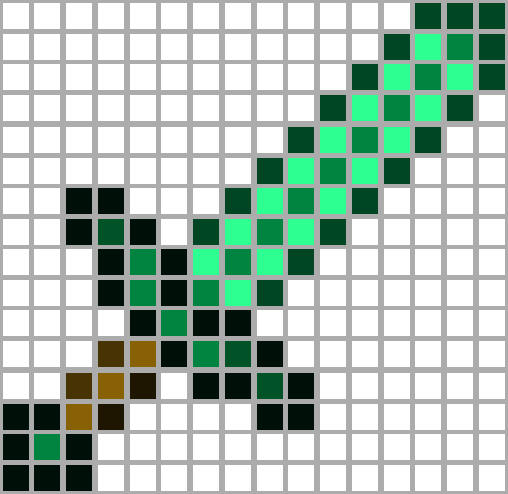
\includegraphics[width=4cm, height=4cm]{Graphics/diamon_sword.png}
	\hspace{1cm}
	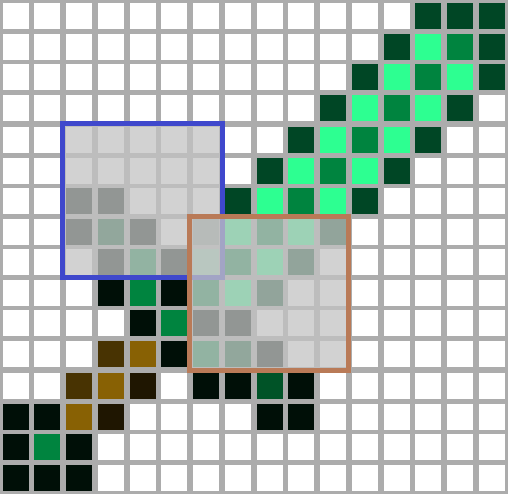
\includegraphics[width=4cm, height=4cm]{Graphics/diamon_sword_with_patches.png}
	\caption{Una imagen de $16 \times 16$ y dos parches de esta tomando $n = 25$.}
	\label{ex:patches}
\end{figure}

En la figura \ref{ex:patches} se ejemplifica visualmente el concepto de parches. Como vemos estos pueden solaparse sin ning\'un problema. Es de inter\'es en el siguiente cap\'itulo el conjunto de todos los parches, incluyendo con solapamientos.

\begin{lemma}\label{le:count_patches}
	La cantidad de parches de una matriz (imagen) incluyendo los solapamientos, para una matriz $A$ de dimensiones $a \times b$, y tomando los parches de $\sqrt{n} \times \sqrt{n}$, es igual a:
	
	\begin{equation}
		(a - \sqrt{n} + 1)(b - \sqrt{n} + 1)
		\label{eq:count_patches}
	\end{equation}
\end{lemma}


\textbf{Demostraci\'on:} tomando como referencia la esquina superior izquierda de un parche, esta solo puede ser ubicada verticalmente en el intervalo de posiciones \\$[1,\; a - \sqrt{n} + 1]$, de lo contrario el parche sobresaldr\'ia de la imagen. An\'alogamente solo puede ser colocado horizontalmente en el intervalo de posiciones $[1,\; b - \sqrt{n} + 1]$. Aplicando el principio combinatorio de la multiplicaci\'on, un parche puede ser ubicado de $(a - \sqrt{n} + 1)(b - \sqrt{n} + 1)$ formas distintas $\blacksquare$.

\begin{lemma}\label{le:count_patches_ieq}
	La cantidad de parches con solapamiento de una matriz A, con $n > 1$, es menor que la cantidad de elementos de la misma.
\end{lemma}

\textbf{Demostraci\'on:} Sea $A$ de $a \times b$; dado que $n > 1$ se cumple la siguiente desigualdad:

\begin{equation}
	\begin{array}{lrcl}
		                &               1 &<& n        \\ 
		\Longrightarrow &               1 &<& \sqrt{n} \\
		\Longrightarrow &   -\sqrt{n} + 1 &<& 0        \\
		\Longrightarrow & a -\sqrt{n} + 1 &<& a        \\
	\end{array}
\end{equation}

An\'alogamente $b -\sqrt{n} + 1 < b$, multiplicando las dos desigualdades obtenemos:

\begin{equation}
	(a - \sqrt{n} + 1)(b - \sqrt{n} + 1) < ab
	\label{eq:count_patches_ieq}
\end{equation}

Por el lema \ref{le:count_patches} la cantidad de parches de A es $(a - \sqrt{n} + 1)(b - \sqrt{n} + 1)$ lo que es menor que $ab$ $\blacksquare$.

\begin{definition}
	El p\'ixel o elemento central de un parche es aquel que se encuentra en una posici\'on prefijada, dicha posici\'on debe ser la misma para todos los parches de una misma imagen.
\end{definition}

\begin{figure}[h]
	\centering
	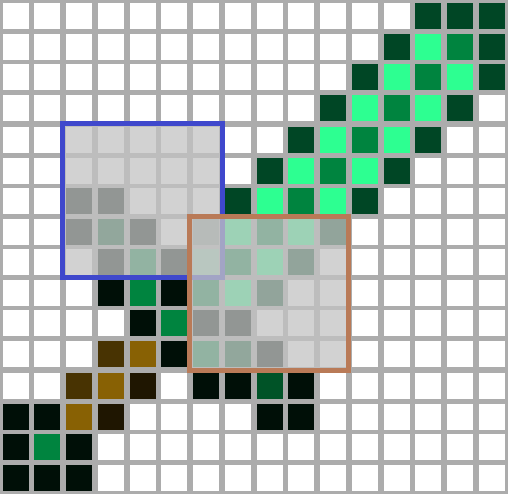
\includegraphics[width=4cm, height=4cm]{Graphics/diamon_sword_with_patches.png}
	\hspace{1cm}
	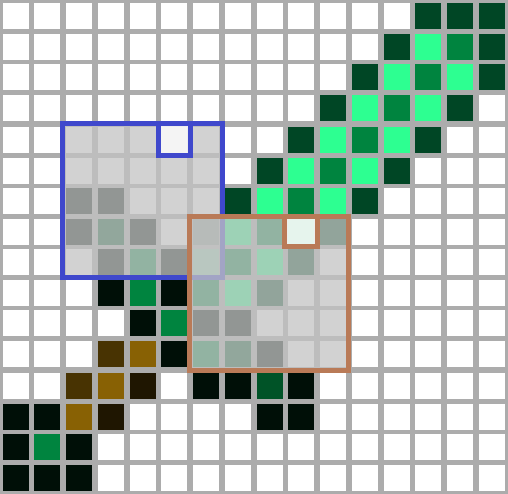
\includegraphics[width=4cm, height=4cm]{Graphics/diamon_sword_with_patches_and_centers.png}
	\caption{Parches con p\'ixel central (marcado en rojo) situado en la posici\'on $4$.}
	\label{ex:patch_center}
\end{figure}

En la figura \ref{ex:patch_center} se muestran los centros de los parches del ejemplo anterior. No debemos confundir el p\'ixel central con aquel que se encuentra en su centro geom\'etrico. La idea de este elemento es para tomarlo como punto de referencia o representativo. Un ejemplo se ve en el cap\'itulo \ref{chapter:SCHEME}, como para aquellos p\'ixles que no se conoce su valor, se usa en cambio el parche del cual ellos son su centro.
\chapter{Esquema de la recuperaci\'on de im\'agenes}\label{chapter:SCHEME}

\section{Esquema inicial}
Planteemos primeramente el esquema principal de esta propuesta para la recuperaci\'on de im\'agenes. Para ello consideremos la siguiente notaci\'on:

\begin{itemize}
	\item $\Z$: matriz que representa la imagen incompleta a recuperar, con dimensiones $N_1 \times N_2$, $N_1N_2 = N$.
	\item $\z$: versión en forma de vector(o señal) de la matriz $\Z$, con dimensiones $N \times 1$.
	\item $\P$: matriz de permutaci\'on de dimensiones $N \times N$.
\end{itemize}

Para obtener la una señal recuperada $\yhat$ a partir de $\z$ se procede de la siguiente forma:

\qquad

\begin{figure}[h]
	\centering
	\begin{equation*}
		\begin{array}[t]{ccccccccc}
		& & \mbox{\small{Permutaci\'on}} & & \mbox{\small{Operador de suavidad}} & & \mbox{\small{Permutaci\'on inversa}} & &\\
		\z & \longrightarrow & \boxed{\P} & \longrightarrow & \boxed{\H} & \longrightarrow & \boxed{\P^{-1}} & \longrightarrow & \yhat \\
		\end{array}
	\end{equation*}
	\caption{Esquema inicial}
	\label{fig:init_scheme}
\end{figure}

\qquad

Se reordenan los elementos de $\z$ seg\'un $\P$, y a la señal resultante $\z^p$ se le aplica un operador de suavidad $\H$ con el cual se obtienen los elementos faltantes, los elementos de dicho resultado se permutan nuevamente a su posici\'on inicial mediante $\P^{-1}$. Dicho vector final ser\'ia $\yhat$. Lo anterior puede expresarse como:

\begin{equation}
\yhat = \P^{-1}\H(\z^p) = \P^{-1}\H(\P\z)
\label{eq:yhat}
\end{equation}

Para comprender mejor lo que se quiere lograr con este procedimiento supongamos que contamos con la imagen real, la versi\'on de $\Z$ con la informaci\'on todos sus p\'ixeles. Aunque en la pr\'actica esta imagen no existe, la utilizaremos para reflejar de forma clara el funcionamiento del esquema inicial (figura \ref{fig:init_scheme}).

\begin{itemize}
	\item $\Y$: matriz de la imagen original, es igual a $\Z$ solo que si tiene el valor de sus p\'ixeles faltantes. 
	\item $\y$: versión en forma de vector(o señal) de la matriz $\Y$.
\end{itemize}

Supongamos que la matriz de permutaci\'on $\P$ tiene la propiedad de que al ser aplicada a $\y$ se obtiene una señal suave $\y^p$. Entonces, dado que $\z^p$ y $\y^p$ solo difieren en los p\'ixeles faltantes de $\Z$, y que $\H(z^p)$ completa la señal, haciéndola suave; se puede esperar que $\yhat$ sea una aproximaci\'on de $\y$. Dicho formalmente:

\begin{equation}
	\def\arraystretch{1.5}
	\begin{array}{lrcl}
	                                           &     \H (\P\z ) &\approx& \P\y        \\ 
	\Longrightarrow                            & P^{-1}\H(\P\z) &\approx& \P^{-1}\P\y \\
	\overset{(\ref{eq:yhat})}{\Longrightarrow} &          \yhat &\approx& \y          \\
	\end{array}
	\label{eq:permutation_smoothness}
\end{equation}

Llegados a este punto las únicas incógnitas son qu\'e operador $\H$ usar, y c\'omo obtener la matriz $\P$. Operadores para suavizar en \textbf{1D} hay varios en la literatura, ya sea los que se usan en interpolaci\'on o filtrado; por el momento dejemos este operador como un superpar\'ametro del algoritmo. Se explicar\'a entonces c\'omo hacer para obtener la permutaci\'on $\P$.

\section{La matriz de permutaci\'on}

El resultado (\ref{eq:permutation_smoothness}) tiene como condici\'on que $\y^p$ sea una señal suave. Para calcular la suavidad de $\y^p$ según (referencia a la formula de suavidad) ser\'ia:

\begin{equation}
\|\y^p\|_{\mathit{TV}} = \sum_{j = 2}^{N}|\y_j^{p} - \y_{j - 1}^{p}|
\label{eq:signal_smoothness}
\end{equation}

La matriz $\P$ que buscamos es tal que minimiza $\|\y^p\|_{\mathit{TV}}$, recordemos que no se cuenta con la señal  $\y$, entonces calcular $|\y_j^{p} - \y_{j - 1}^{p}|$ solo es posible cuando ambos elementos est\'an en la imagen incompleta $\Z$, lo que significa que conocemos su valor. Para encontrar la distancia entre dos p\'ixeles de $\Z$ (arbitrariamente de si se conoce su valor o no) usaremos sus parches de la siguiente manera:

\begin{equation}
|\y_j^{p} - \y_{j - 1}^{p}| \equiv \omega(\x_j^p,\; \x_{j - 1}^p)
\label{eq:omega_mean}
\end{equation}

Donde $\x_j^p$ denota el parche de $\Z$ cuyo p\'ixel central es denotado por $\z_j^p$. Y $\omega$ es una funci\'on de distancia definida sobre los parches la cual cumple que para cualesquiera dos parches, proximidad entre ellos sugiere proximidad entre sus p\'ixeles centrales, justo como se expresa en (\ref{eq:omega_mean}). Luego, el problema de minimizar $\|\y^p\|_{\mathit{TV}}$ por (\ref{eq:signal_smoothness}) y (\ref{eq:omega_mean}) es equivalente a minimizar:

\begin{equation}
\|\X^p\|_{\mathit{TV}} = \sum_{j = 2}^{N}\omega(\x_j^{p},\; \x_{j - 1}^{p})
\label{eq:path_smoothness}
\end{equation}

Donde $\X$ denota el vector de los parches de $\Z$ y $\X^p$ una permutaci\'on de $\X$ dada por una matriz $\P$. En conclusi\'on: la matriz $\P$ que buscamos es aquella  que minimiza $\|\X^p\|_{\mathit{TV}}$. Ahora bien, lo anterior se puede replantear de la siguiente forma. Si consideramos el grafo ponderado cuyos nodos son todos los parches de $\Z$ y la arista que une cada par de nodos $\x_i,\;\x_j$ tiene peso $\omega(\x_i,\; \x_j)$; debemos resolver una instancia del problema \textbf{NP}-completo del viajero, conocido como \TSP (del ingl\'es \textit{traveling salesman problem}) buscando un camino que comience en un parche cualquiera, pase por el resto de los parches una \'unica vez y cuya longitud es m\'inima.

\section{Algoritmo de reordenamiento de parches}

No se conoce ningún algoritmo con complejidad temporal polinomial para resolver \TSP, con lo cual en favor de lograr la eficiencia del esquema de la recuperaci\'on se tom\'o un algoritmo que encuentra una soluci\'on aproximada. El camino de parches que encuentra puede no ser el de m\'inima longitud, pero se garantiza que ser\'a de los menores. En cambio esta soluci\'on aproximada si se encuentra en un tiempo polinomial, que en este caso ser\'a lineal con respecto a la cantidad de parches o sea $O(\dim(\X))$.

Primeramente, se selecciona aleatoriamente un parche $\x_{j_0}$ por el cual comienza el camino. Luego se va iterando poniendo en cada paso un parche hasta completar el camino. En la iteraci\'on $k$ se explora la vecindad de tamaño $\B \times \B$ en la matriz $\Z$ alrededor del parche $\x_{j_{k - 1}}$ (que es el \'ultimo que se ha puesto). Ahora bien, existen dos casos:

\begin{itemize}
\item Todos los parches en esta vecindad ya están en el camino: se busca fuera de la vecindad los dos parches $\x_a,\; \x_b$ que no pertenecen al camino y cuyas distancias $\omega$ a $\x_{j_{k - 1}}$ son las dos menores.

\item Si existen parches disponibles en esa vecindad: se buscan de forma an\'aloga los parches $\x_a,\; \x_b$, esta vez dentro de la vecindad
\end{itemize}

Claramente si no es posible encontrar dos menores porque solo hay un parche disponible, entonces $\x_{j_k}$ ser\'ia ese \'unico parche. En cambio si se tienen $\x_a$ y $\x_b$ entonces:

\begin{equation}
\x_{j_k} = \left\{
	\begin{array}{ccc}
	\x_a &\mbox{con probabilidad}& p_a = \alpha e^{-\frac{\omega(\x_{j_{k - 1}},\; \x_a)}{\epsilon}}\\
	\x_b &\mbox{con probabilidad}& p_b = \alpha e^{-\frac{\omega(\x_{j_{k - 1}},\; \x_b)}{\epsilon}}\\
	\end{array}
\right.
\end{equation}

Donde $\alpha$ es tal que $p_a + p_b = 1$ y $\epsilon$ es un valor ajustable. Finalmente el conjunto de \'indices $\{j_i\}$ del camino de parches define la permutaci\'on $\P$ que buscamos. El pseudoc\'odigo se muestra en el algoritmo \ref{al:PRA}.

\begin{algorithm}
	\DontPrintSemicolon % Some LaTeX compilers require you to use \dontprintsemicolon instead
	\KwIn{Todos los parches de la imagen: $\{\mathbf{x}_i\}_{i = 1}^M$}
	\KwOut{$\Omega$, reordenamiento del conjunto $ \{1,\;2,\;...,\;M\}$}
	$\Omega(1) \gets$ Un entero aleatorio en el intervalo $[1,\; M]$\;
	\For{$k \gets 1$ \textbf{to} $M - 1$} {
		$A_k \gets $ Conjuto de los \'indices de los $B \times B$ parches alrededor de $\x_{\Omega(k)}$\;
		\If{$|A_k \setminus \Omega| = 1$} {
			$\Omega(k + 1) \gets A_i \setminus \Omega$\;
		}
		\Else{
			\If{$|A_k \setminus \Omega| \ge 2$}{
				Encontrar $\x_a, \x_b$ los parches m\'as ceranos a $\x_{\Omega(k)}$ tales que $a, b \in |A_k \setminus \Omega|$\;
			}
			\Else{
				Encontrar $\x_a, \x_b$ los parches m\'as ceranos a $\x_{\Omega(k)}$ tales que $a, b \notin \Omega$\;
			}
			$\Omega(k + 1) \gets \left\{
				\begin{array}{ccc}
				\x_a &\mbox{con probabilidad}& p_a = \alpha e^{-\frac{\omega(\x_{j_{k - 1}},\; \x_a)}{\epsilon}}\\
				\x_b &\mbox{con probabilidad}& p_b = \alpha e^{-\frac{\omega(\x_{j_{k - 1}},\; \x_b)}{\epsilon}}\\
				\end{array}
			\right.$\;
		}
	}
	\Return{$\Omega$}\;
	\SetAlgoRefName{1}
	\caption{Reordenamiento de los parches}
	\label{al:PRA}
\end{algorithm}

\section{Trabajo con subim\'agenes}
Tomando como $n$ el tamaño de los parches en este procedimiento, tenemos por (referencia a cap 1) que la cantidad de parches de la matriz $\Z$ es: 

\begin{equation}
N_p = (N_1 - \sqrt{n} + 1)(N_2 - \sqrt{n} + 1)
\label{eq:patches}
\end{equation}

Es claro que $n > 1$, pues los parches cubren pequeñas zonas de p\'ixeles, con lo cual se cumple la siguiente desigualdad:

\begin{equation}
	\begin{array}{lrcl}
	                &                 1 &<& n        \\ 
	\Longrightarrow &                 1 &<& \sqrt{n} \\
	\Longrightarrow &     -\sqrt{n} + 1 &<& 0        \\
	\Longrightarrow & N_1 -\sqrt{n} + 1 &<& N_1      \\
	\end{array}
\end{equation}

An\'alogamente $N_2 -\sqrt{n} + 1 < N_2$, multiplicando estas dos desigualdades obtenemos que:

\begin{equation}
	\begin{array}{lrcl}
	                & (N_1 - \sqrt{n} + 1)(N_2 - \sqrt{n} + 1) &<& N_1N_2 \\ 
	\Longrightarrow &                                      N_p &<& N      \\
	\label{eq:patches_ineq}
	\end{array}
\end{equation}

La cantidad de parches $N_p$ de $\Z$ es menor que el tamaño del vector $\z$, luego las dimensiones de la matriz $\P$ obtenidas con algoritmo \ref{al:PRA} son de $N_p \times N_p$; lo que implica que el esquema inicial (figura \ref{fig:init_scheme}) solo ser\'ia aplicables a señales de tamaño $N_p \times 1$.

\begin{figure}[h]
	\[\Z = \left(
	\begin{matrix}
	a & b & c & d\\\cline{2-3}
	e & \multicolumn{1}{|c}{f} & \multicolumn{1}{c|}{g} & h\\
	i & \multicolumn{1}{|c}{j} & \multicolumn{1}{c|}{k} & l\\\cline{2-3}
	m & n & o & p\\
	\end{matrix}
	\right)
	\qquad\X = \left(
	\begin{matrix}\cline{5-5}
	a & b & c & e & \multicolumn{1}{|c|}{f} & g & i & j & k\\
	b & c & d & f & \multicolumn{1}{|c|}{g} & h & j & k & l\\
	e & f & g & i & \multicolumn{1}{|c|}{j} & k & m & n & o\\
	f & g & h & g & \multicolumn{1}{|c|}{k} & l & n & o & p\\\cline{5-5}
	\end{matrix}
	\right)
	\]
\end{figure}

Tengamos en cuenta que la subimagen formada por los p\'ixeles centrales de cada parche es una señal de tamaño $N_p$, entonces podr\'iamos aplicarle el esquema (figura \ref{fig:init_scheme}) para recuperar por completo esa subimagen. Considerando todos los posibles centros para los parches, tendremos un total de $n$ subim\'agenes (referencia al capitulo 1). Si recuperamos cada una de estas usando el esquema inicial, podemos usar esas subim\'agenes recuperadas para colocarlas en su posición natural en $\Z$, est\'a claro que todas se solapan, pero para ello promediamos los p\'ixeles solapados, y así se formar\'ia una imagen completa recuperada.  

Si vemos al vector de parches $X$ como una matriz, poniendo los parches como columnas, entonces cada fila de esta matriz es una submimagen en forma de vector. Tal y como muestra es siguiente ejemplo

\begin{equation}
	\z\;\left\{
	\def\arraystretch{2.2}
	\begin{array}{ccccccccc}
		\longrightarrow & \boxed{\P_1} & \longrightarrow & \boxed{\H} & \longrightarrow & \boxed{\P_1^{-1}} & \longrightarrow \\
		\longrightarrow & \boxed{\P_2} & \longrightarrow & \boxed{\H} & \longrightarrow & \boxed{\P_2^{-1}} & \longrightarrow \\
		\longrightarrow & \huge\vdots &  & \huge\vdots &  & \huge\vdots & \longrightarrow & \\
		\longrightarrow & \boxed{\P_K} & \longrightarrow & \boxed{\H} & \longrightarrow & \boxed{\P_K^{-1}} & \longrightarrow
	\end{array}
	\right\}\;\oplus\longrightarrow\boxed{\times\frac{1}{K}}\longrightarrow\yhat
\end{equation}

%	Ejemplo de algoritmo:
%	
%	\begin{algorithm}
%	    \caption{Algoritmo de Arnoldi para construir una base ortonormal del subespacio de Krylov $\mathcal{K}_\mf(\tau A,b)$}
%	    \label{alg:Arnoldi}
%	    \KwIn{Matriz $A\in \mathbb{R}^{d\times d}$, vector $b\in \mathbb{R}^{d}$ y constante $\tau$}
%	    \KwOut{Base ortonormal $\{v_1,v_2,\ldots,v_\mf,v_{\mf+1}\}$ de $K_\mf(\tau A,b)$ y matriz de Hessenberg $H_\mf=V_\mf^{\intercal}\tau A V_\mf $,
%	        donde $V_{\mf+1}=[v_1\,v_2\,\cdots \,v_\mf\,v_{\mf+1}]\in \mathbb{R}^{d\times \mf+1}$, $breakdown$ }
%	    $breakdown=false$\\
%	    $v_1=b/\lVert b \rVert_2$\\
%	    \For{ $j=1,2,\ldots,\mf$ }{
%	        $w_j=\tau A v_j$\\
%	        \For{ $i=1,\ldots,j$}{ 
%	            $\hf_{ij}=\langle w_j,v_i \rangle$\\
%	            $w_j=w_j-\hf_{ij}v_i$       
%	        }
%	        $\hf_{j+1,i}=\lVert w_j \rVert_2$\\
%	        \eIf(\tcp*[h] \emph{Break Down}\label{alg:breakdown}){$\hf_{j+1,i}<2\epsilon_{mach}$}{
%	            $\mf_{cut}=j$\\
%	             $breakdown=true$\\
%	            Stop
%	        }{
%	            $v_{j+1}=w_j/\hf_{j+1,i}$
%	        }
%	    }
%	\end{algorithm}



\chapter{Implementaci\'on}\label{chapter:code}

En este capítulo se discute acerca de la implementación del algoritmo \ref{al:PRA} presentado en el Capítulo \ref{chapter:scheme} y del esquema final de la restauraci\'on presentado en el epígrafe \ref{sec:final_scheme}. El c\'odigo fuente de la implementaci\'on puede consultarse en el siguiente repositorio: \url{https://github.com/danielgpz/image-inpainting-sop.git}.

\section{Tecnolog\'ias utilizadas}
Todos los algoritmos y el c\'odigo fuente en general han sido implementados en el lenguaje de programaci\'on \texttt{Python3}, específicamente en su versi\'on \texttt{python 3.7.3}. Para el trabajo con los archivos de im\'agenes digitales, como son las operaciones de \textit{lectura}\footnote{Operaci\'on de cargar determinados datos en un disco duro o dispositivo de almacenamiento hacia la memoria \textbf{RAM}.} y \textit{escritura}\footnote{Operaci\'on inversa de la lectura, copiar determinados datos de la memoria hacia el dispositivo de almacenamiento.} se us\'o la librer\'ia \texttt{OpenCV}\footnote{Por sus siglas en ingles \textit{Open Source Computer Vision Library}: librer\'ia de c\'odigo abierto para visi\'on por computadoras.} en su versi\'on \texttt{cv2 4.2.0}. \texttt{OpenCV} es un \textit{software} librer\'ia de c\'odigo abierto\footnote{D\'igase de aquellos programas cuyo c\'odigo fuente no est\'a oculto o encriptado. Cualquier usuario es libre de verificarlo y contribuir al mismo.} que se utiliza para visi\'on por computadoras e Inteligencia Artificial. La misma contiene m\'as de $2500$ algoritmos optimizados que comprenden tanto los cl\'asicos como los del estado del arte en los dos campos anteriormente mencionados. Utilizando los m\'etodos \fbox{\texttt{cv2.imread}} y \fbox{\texttt{cv2.imwrite}} de esta librer\'ia se logra la lectura y la escritura respectivamente de las im\'agenes digitales. Estos permiten adem\'as obtener la representaci\'on matricial asociada. Ambas funciones soportan el uso de la mayor\'ia de los formatos para imágenes matriciales como son \texttt{.bmp}, \texttt{.jpg}, \texttt{.png}, \texttt{.tif}, entre otros, y cuentan con la opción de usar el mapa de color \RGB/ o la escala de grises.

Para el trabajo con matrices, vectores, otros elementos y operaciones matem\'aticas se hace uso de la librer\'ia \texttt{NumPy} en su versi\'on \texttt{numpy 1.17.4}. Esta librer\'ia es considerada la m\'as ampliamente usada del paquete científico de \texttt{Python}. La misma provee las herramientas para tratar con las matrices obtenidas mediante \texttt{OpenCV} y facilita la realización de transformaciones y operaciones tanto elementales como avanzadas. Adem\'as de las matrices, se usa tambi\'en el m\'odulo \fbox{\texttt{numpy.random}} \'util para el trabajo con variables aleatorias. \texttt{NumPy} es r\'apida y eficiente, conocida por estar mayormente implementada en el lenguaje \texttt{C} lo que ayuda a evitar los procesos lentos y cargados en memoria, t\'ipicos de \texttt{Python}.

\texttt{SciPy} es otra de las librer\'ias m\'as conocidas del paquete científico, de la que tambi\'en se hace uso en este trabajo. La versión usada es \texttt{scipy 1.3.2}. De esta se toma el m\'odulo \fbox{\texttt{scipy.interpolate}} el cual contiene, entre otras, una funci\'on para realizar la interpolaci\'on por \textit{splines} c\'ubicos. Finalmente, con el objetivo de optimizar el tiempo de ejecuci\'on de los esquemas y algoritmos presentados en el Cap\'itulo \ref{chapter:scheme} se utiliza el m\'odulo \texttt{multiprocessing}. Este paquete soporta la ejecuci\'on de procesos concurrentes, de una forma similar al m\'odulo \texttt{threading}, con la gran diferencia de que estos procesos s\'i corren en diferentes n\'ucleos de la \textbf{CPU}\footnote{Por sus siglas en ingl\'es \textit{Central Processing Unit}: unidad central de procesamiento.} \cite{o2008brief}. Este m\'odulo resulta de utilidad para lograr la paralelizaci\'on de los esquemas de restauraci\'on presentados, que tal como sus gr\'aficos muestran (figuras \ref{fig:subimage_scheme} y \ref{fig:final_scheme}), sus partes pueden ser realizadas de forma independiente.

\section{El m\'odulo \texttt{ImageInpainting}}\label{sec:imageinpainting_module}

Para lograr una mejor organizaci\'on y diseño de la implementaci\'on del esquema de restauraci\'on, la misma se cre\'o en forma de m\'odulo local de \texttt{Python}, el cual se nombr\'o \texttt{ImageInpainting}. Este constituye uno de los aportes de este trabajo en la implementación. Cada una de sus funcionalidades fueron encapsuladas en 4 archivos distintos:
\begin{itemize}
	\item \texttt{images.py}: archivo que contiene los m\'etodos para la lectura y escritura de las im\'agenes digitales y su conversi\'on a matrices de \texttt{NumPy}.
	\item \texttt{pra.py}: solo contiene un \'unico m\'etodo con la implementaci\'on del algoritmo \ref{al:PRA}.
	\item \texttt{operators.py}: contiene las implentaciones del operador de suavidad $\H$ y la funci\'on de distancia entre parches $\omega$.
	\item \texttt{inpainting.py}: contiene la implementaci\'on de una clase para modelar el concepto de imagen corrupta o con p\'ixeles faltantes.
\end{itemize}

A continuaci\'on se da una explicaci\'on m\'as detallada por cada uno de los archivos:
\begin{enumerate}
	\item Archivo \texttt{images.py}, en este se encuentran las siguientes funciones:
	\begin{itemize}
		\item \fbox{\lstinline|read_image_as_arrays(location, rgb=False, dtype=int)|}
		
		M\'etodo que por medio de \texttt{cv2.imread} lee la imagen digital del disco duro, y la transforma a uno o tres arreglos bidimensionales de \texttt{numpy}. \underline{Par\'ametros}:
		\begin{itemize}
			\item \texttt{location}: tipo \texttt{str}, direcci\'on donde se almacena la im\'agen a leer en el disco.
			\item \texttt{rgb}: tipo \texttt{bool}, indica si la imagen debe ser le\'ida como \RGB/ o escala de grises. En el primer caso, se generar\'an 3 arreglos uno por cada canal. En el caso de la escala de grises, un \'unico arreglo. Valor por defecto: \texttt{False}.
			\item \texttt{dtype}: tipo \texttt{type}, tipo datos con que se interpretar\'an los p\'ixeles. Usar \texttt{int} para el intervalo usual de $[0,\; 255]$. Usar \texttt{bool} para interpretar la imagen como una m\'ascara. Valor por defecto: \texttt{int}.
		\end{itemize}
		\underline{Retorna}: una tupla de arreglos, cada arreglo representando uno de los canales de la imagen, 3 para \texttt{rgb=True} y 1 para \texttt{rgb=False}.
		
		\item \fbox{\lstinline|read_image_as_mask(location, true_value=0)|}
		
		 M\'etodo que por medio de \texttt{cv2.imread} lee la imagen digital del disco duro, y la interpreta como una m\'ascara. \underline{Par\'ametros}:
		\begin{itemize}
			\item \texttt{location}: tipo \texttt{str}, direcci\'on donde se almacena la im\'agen m\'ascara en el disco.
			\item \texttt{true\_value}: tipo \texttt{int}, indica el valor de los p\'ixeles que se tomar\'an como \texttt{True} en la m\'ascara que se retorna. Valor por defecto \texttt{0}.
		\end{itemize}
		\underline{Retorna}: un arreglo bidimensional de booleanos, la m\'ascara leída.
		
		\item \fbox{\lstinline|save_arrays_as_image(arrays, location, rgb=False)|}
		
		M\'etodo que, usando \texttt{cv2.imwrite}, almacena la imagen digital en el disco duro. Dicha imagen es la representada por el par\'ametro \texttt{arrays}. \underline{Par\'ametros}:
		\begin{itemize}
			\item \texttt{arrays}: tipo \texttt{tuple}, tupla de uno o tres arreglos bidimensionales que representan los canales de la imagen a alamacenar.
			\item \texttt{location}: tipo \texttt{str}, direcci\'on que indica donde debe ser almacenada la imagen en el disco duro.
			\item \texttt{rgb}: tipo \texttt{bool}, tipo de imagen a almacenar, en caso de \texttt{True} se usan los tres arreglos representando en ese orden cada uno de los canales \RGB/. Si no, se toma solo el primero. Valor por defecto: \texttt{False}. 
		\end{itemize}
		\underline{Retorna}: \texttt{None}. No tiene valor de retorno, se considera un m\'etodo \textit{void}.
	\end{itemize}
	
	\item Archivo \texttt{pra.py}, el cual contiene la implementaci\'on del algoritmo \ref{al:PRA}:
	\begin{itemize}
		\item \fbox{\lstinline|patch_reordering(shape, patches, B, epsilon, omega)|}
		
		M\'etodo implementado seg\'un el pseudoc\'odigo del algoritmo \ref{al:PRA}. \underline{Par\'ametros}:
		\begin{itemize}
			\item \texttt{shape}: tipo \texttt{tuple}, tupla de 2 elementos que denota la dimensi\'on de cada subimagen, en otras palabras ($N_1 - \sqrt{n} + 1)$ y $(N_2 - \sqrt{n} + 1)$.
			\item \texttt{patches}: tipo \texttt{numpy.ndarray}, arreglo bidimensional que representa la matriz $X^\intercal$, cada fila es un parche vectorizado. Los parches se toman columna por columna de arriba hacia abajo.
			\item \texttt{B}: tipo \texttt{int}, entero que representa el tamaño de la vecindad a explorar en cada iteraci\'on.
			\item \texttt{epsilon}: tipo \texttt{float}, n\'umero de punto flotante que se atribuye a $\epsilon$.
			\item \texttt{omega}: tipo \texttt{function}, funci\'on que toma como par\'ametros dos arreglos de tipo \texttt{numpy.array} y retorna un \texttt{float} que es la distancia entre los parches vectorizados que representan. Equivalente de la funci\'on $\omega$.
		\end{itemize}
		\underline{Retorna}: una tupla de 2 arreglos, el primero contiene los \'indices que definen la permutaci\'on generada y el segundo los de la permutaci\'on inversa.
	\end{itemize}
	
	\item Archivo \texttt{operators.py}, que define sus funciones de la siguiente forma:
	\begin{itemize}
		\item \fbox{\lstinline|mean_of_squared_differences(patch1, patch2)|}
		
		M\'etodo para calcular la distancia entre parches seg\'un (\ref{eq:omega}). \underline{Par\'ametros}:
		\begin{itemize}
			\item \texttt{patch1}, \texttt{patch2}: tipo \texttt{numpy.array}, arreglos que representan un parche en forma de vector.
		\end{itemize}
		\underline{Retorna}: un flotante, la distancia entre \texttt{parch1} y \texttt{patch2}, \texttt{-1} en caso de ser disjuntos en cuanto a sus p\'ixeles no faltantes.
		
		\item \fbox{\lstinline|cubic_spline(signal, mask)|}
		
		M\'etodo para aplicar el operador de suavidad usando interpolaci\'on por \textit{splines} c\'ubicos. \underline{Par\'ametros}:
		\begin{itemize}
			\item \texttt{signal}: tipo \texttt{numpy.array}, arreglo de elementos que representa una señal a interpolar.
			\item \texttt{mask}: tipo \texttt{numpy.array}, arreglo de elementos booleanos, de mismo tamaño que \texttt{signal} y contiene \texttt{False} en aquella posiciones donde ocurre un elemento faltante de \texttt{signal}.
		\end{itemize}
		\underline{Retorna}: un arreglo de mismo tamaño que \texttt{signal} resultado de la interpolaci\'on en cada una de las posiciones del arreglo \texttt{signal}.
	\end{itemize}
	
	\item Archivo principal \texttt{inpainting.py}, el cual contiene las funcionalidades para realizar el esquema completo de la restauraci\'on haciendo uso de los m\'etodos implementados en \texttt{images.py},  \texttt{pra.py} y \texttt{operators.py}.
	Para modelar el concepto de una imagen con p\'ixeles faltantes se implement\'o:
	\begin{lstlisting}
class CorruptedImage:
	def __init__(self, location: str, mask=None, rgb=False, 
				corrupt_prob=4/5): ...
	
	def save(self, location: str): ...
	
	def inpainting(self, K=10, sqrt_n=16, B=9, epsilon=10**4,
			H=cubic_spline, omega=mean_of_squared_differences): ...
	\end{lstlisting}
	\begin{itemize}
		\item \fbox{\lstinline|__init__(self, location, mask=None, rgb=False, corrupt_prob=4/5)|}
		
		M\'etodo inicializador de instancia para la clase \texttt{CorruptedImage}. Se carga la m\'ascara y la imagen, la cual se divide en canales. \underline{Par\'ametros}:
		\begin{itemize}
			\item \texttt{location}: tipo \texttt{str}, direcci\'on en el disco duro de la imagen digital a recuperar. Los canales de la misma se obtienen mediante el m\'etodo \texttt{read\_image\_as\_arrays} y se almacenan en el atributo \texttt{self.channels}.
			\item \texttt{mask}: tipo \texttt{numpy.ndarray}, arreglo booleano bidimensional de mimas dimensi\'on que la imagen cargada. M\'ascara que indica con \texttt{False} los p\'ixeles faltantes. Se almacena en el atributo \texttt{self.mask}. Valor por defecto: \texttt{None}.
			\item \texttt{rgb}: tipo \texttt{bool}, par\'ametro que indica si la imagen debe ser cargada como \RGB/ o escala de grises. Valor por defecto: \texttt{False}.
			\item \texttt{corrupt\_prob}: tipo \texttt{float}, valor en el intervalo $[0,\; 1]$. En caso de que \texttt{mask} sea \texttt{None}, se genera una m\'ascara de forma aleatoria asignando \texttt{False} en cada posici\'on con probabilidad de dicho valor. Valor por defecto: \texttt{4/5}. 
		\end{itemize}
		\underline{Retorna}: la instancia creada.
		
		\item \fbox{\lstinline|save(self, location)|}
		
		M\'etodo de instancia para almacenar el estado actual de la imagen en el disco duro. \underline{Par\'ametros}:
		\begin{itemize}
			\item \texttt{location}: tipo \texttt{str}, direcci\'on en el disco duro d\'onde almacenar la imagen. 
		\end{itemize}
		\underline{Retorna}: \texttt{None}, es un m\'etodo \textit{void}.
		
		\item \fbox{\lstinline|inpainting(self, K=10, sqrt_n=16, B=9, epsilon, H, omega)|}
		
		M\'etodo para realizar el esquema de restauraci\'on (figura \ref{fig:final_scheme}) a cada uno de los canales almacenados en el atributo de la instancia \texttt{self.channels}. \underline{Par\'ametros}:
		\begin{itemize}
			\item \texttt{K}: tipo \texttt{int}, cantidad de permutaci\'ones diferentes a usar en el esquema, las cuales se obtienen usando el m\'etodo \texttt{patch\_reordering}. Valor por defecto \texttt{10}.
			\item \texttt{sqrt\_n}: tipo \texttt{int}, valor de $\sqrt{n}$ que indica que los parches tienen dimensi\'on $\sqrt{n} \times \sqrt{n}$. Valor por defecto \texttt{16}.
			\item \texttt{B}: tipo \texttt{int}, tamaño de la vecindad a usar en los llamados al m\'etodo \texttt{patch\_reordering}. Valor por defecto \texttt{9}.
			\item \texttt{epsilon}: tipo \texttt{float}, valor de $\epsilon$ a usar en los llamados al m\'etodo \\\texttt{patch\_reordering}. Valor por defecto \texttt{10000}.
			\item \texttt{H}:tipo \texttt{function}, m\'etodo que recibe dos arreglos y retorna una tercero, todos de igual tamaño. El arreglo retornado debe ser el resultado de aplicarle determinado operador de suavidad a la señal representada por el primero, usando el segundo como m\'ascara para definir los elementos corruptos. Valor por defecto, m\'etodo \texttt{cubic\_spline}.
			\item \texttt{omega}: tipo \texttt{function}, m\'etodo que representa la funci\'on $\omega$ a usar en los llamados al m\'etodo \texttt{patch\_reordering}. Valor por defecto, el m\'etodo \texttt{mean\_of\_squared\_differences}.
		\end{itemize}
		\underline{Retorna}: \texttt{None}, es un m\'etodo \textit{void}.
	\end{itemize}
\end{enumerate}

\section{\textquestiondown C\'omo usar el m\'odulo \texttt{ImageInpainting}?}\label{sec:module_how_to_use}
Se supone que se tiene una imagen y otra de igual dimensión en forma de m\'ascara. Considérese el ejemplo de  \texttt{woman\_blonde.tif} y \texttt{mask.tif} (ver figura \ref{fig:woman_blonde}). Para realizar la restauraci\'on de la imagen se procede como el en siguiente ejemplo:
\begin{figure}[H]
	\centering
	\subfigure[\texttt{woman\_blonde.tif}]{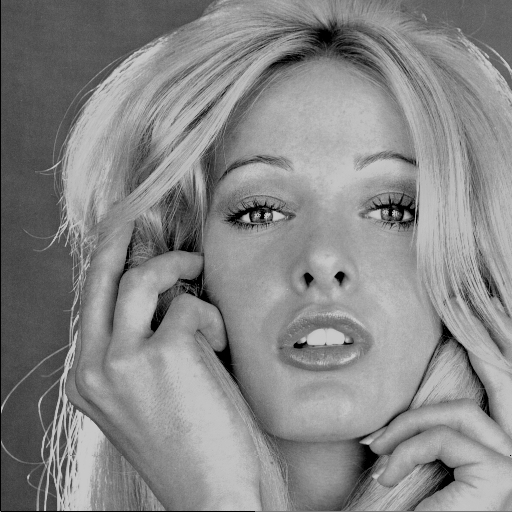
\includegraphics[width=.20\linewidth]{Graphics/Examples/woman_blonde.png}}\qquad
	\subfigure[\texttt{mask.tif}]{\includegraphics[width=.20\linewidth]{Graphics/Examples/mask.tif}}
	\caption{La imagen y su m\'ascara.}
	\label{fig:woman_blonde}
\end{figure}

\begin{lstlisting}
from ImageInpainting import CorruptedImage, read_image_as_mask

# Leyendo la m'ascara y la imagen, luego guardando la imagen corrupta
mask = read_image_as_mask('mask.tif')
im = CorruptedImage('woman_blonde.tif', mask)
im.save('woman_blonde_c.tif')

# Primera restauraci'on con K=10, sqrt_n=5, B=6, epsilon=10000 
im.inpainting(sqrt_n=5, B=6, epsilon=10**4)
im.save('woman_blonde_r1.tif')

# Secunda restauraci'on con K=10, sqrt_n=4, B=7, epsilon=1000000
im.inpainting(sqrt_n=4, B=7, epsilon=10**6)
im.save('woman_blonde_r2.tif')

# Tercera restauraci'on con K=10, sqrt_n=4, B=8, epsilon=100000000 
im.inpainting(sqrt_n=4, B=8, epsilon=10**8)
im.save('woman_blonde_r3.tif')
\end{lstlisting}
La ejecuci\'on de dicho programa genera la versi\'on de la imagen original corrupta seg\'un la m\'ascara, y las 3 im\'agenes restauradas (ver figura \ref{fig:inpainting_woman_blonde}).
\begin{figure}[H]
	\centering
	\subfigure[\texttt{woman\_blonde\_c.tif}]{\includegraphics[width=.23\linewidth]{Graphics/Examples/woman_blonde_corrupted.tif}}\\
	\subfigure[\texttt{woman\_blonde\_r1.tif}]{\includegraphics[width=.23\linewidth]{Graphics/Examples/woman_blonde_iteration_1.tif}}
	\subfigure[\texttt{woman\_blonde\_r2.tif}]{\includegraphics[width=.23\linewidth]{Graphics/Examples/woman_blonde_iteration_2.tif}}
	\subfigure[\texttt{woman\_blonde\_r3.tif}]{\includegraphics[width=.23\linewidth]{Graphics/Examples/woman_blonde_iteration_3.tif}}
	\caption{En ese orden: imagen corrupta y las im\'agenes restauradas.}
	\label{fig:inpainting_woman_blonde}
\end{figure}
Finalmente, se ha de destacar que el diseño de la clase \texttt{CorruptedImage} favorece el poder realizar restauraciones consecutivas, cada una usando los resultados de la anterior. Cada vez que se llama al m\'etodo de instancia \texttt{inpainting}, el mismo actualiza cada canal de la imagen con los nuevos p\'ixeles restaurados. Esto tiene como consecuencia que en la mayor\'ia de los casos una segunda restauraci\'on tiene mejor calidad que una primera con los mismos par\'ametros. N\'otese que en el ejemplo anterior se realizan 3 restauraciones consecutivas, m\'as adelante se demuestra la efectividad de esta estrategia.

\section{Paralelizaci\'on y herramientas para la experimentaci\'on}

Como se muestra en la figura \ref{fig:final_scheme} del esquema final, se deben realizar $K$ restauraciones del tipo esquema con subim\'agenes, y promediar los resultados en una restauraci\'on final. La forma natural es llevar a cabo las restauraciones iterativamente una despu\'es de la otra. Teniendo en cuenta que los resultados de estas $K$ restauraciones no son dependientes, surge la idea de poder ejecutarlas de forma concurrente. Por lo tanto se decide aplicar la paralelizaci\'on en ese nivel del esquema. Se utiliz\'o el tipo \fbox{\texttt{multiprocessing.Pool}} el cual modela un contenedor de procesos que se ejecutan en paralelo. El mismo permite agregar procesos nuevos u obtener el resultado de uno que culmina. Se comienza agregando los procesos de las 3 primeras restauraciones del tipo esquema con subim\'agenes. Luego, en todo momento se estar\'an ejecutando un m\'aximo de 3 procesos en paralelo. En la medida en que alguno culmine, se almacena su resultado y se agrega el siguiente proceso. As\'i sucesivamente hasta realizar las $K$ restauraciones. Esta estrategia reduce el tiempo de ejecución en alrededor de tres veces respecto a la versión sin concurrencia.

Por otro lado, para facilitar la tarea de experimentaci\'on y comprobaci\'on de la restauraci\'on con determinado volumen de im\'agenes se implement\'o \texttt{experiment.py}, haciendo uso de el m\'odulo \texttt{ImageInpainting}. Dicho programa automatiza el proceso de cargar un conjunto im\'agenes, aplicarles la restauraci\'on y almacenar los resultados. El mismo debe proveerse de una descripci\'on simple del experimento a realizar, tal como, la lista de im\'agenes, sus m\'ascaras, cantidad de restauraciones a realizar y qu\'e valores asignar a los par\'ametros en cada caso. Para realizar una evaluaci\'on de los resultados de la experimentaci\'on se hace uso de otras herramientas que ofrece \texttt{OpenCV}. Entre ellas se emplea la implementaci\'on para la medida \textbf{PSNR} \cite{korhonen2012peak} en el Cap\'itulo \ref{chapter:results}, el m\'etodo \fbox{\texttt{cv2.PSNR}}. Tambi\'en se utiliza la funci\'on \fbox{\texttt{cv2.inpainting}} que realiza dos tipos diferentes de restauraci\'on de im\'agenes, los cuales permiten establecer una comparación de la efectividad de estas con la de la estrategia  propuesta en este trabajo.
\chapter{Experimentaci\'on y resultados}\label{chapter:results}
En este cap\'itulo se muestran los resultados de la experimentaci\'on realizada con el esquema de restauraci\'on propuesto en el Cap\'itulo \ref{chapter:scheme}, sobre una serie de im\'agenes digitales tomadas de ciertas colecciones de inter\'es. La implementaci\'on usada es la presentada en el Cap\'itulo \ref{chapter:code}, donde adem\'as se sugiri\'o la estrategia de realizar restauraciones consecutivas que aprovechan la restauraci\'on anterior. La efectividad de la estrategia mencionada se mide de conjunto con la calidad de las restauraciones. Con el objetivo de establecer comparaciones, se realizaron otros dos tipos de restauraciones sobre las mismas im\'agenes. Para distinguir del resto la restauraci\'on propuesta en este trabajo, se usan en su lugar las siglas \SOP/ a modo de abreviatura.

Como primera restauraci\'on de referencia se cuenta con el trabajo realizado por Alexandru Telea en 2004 \cite{telea2004image}. Como se mencion\'o brevemente en la Introducci\'on, esta restauraci\'on se basa en el m\'etodo \textit{fast marching}. La idea principal es propagar la informaci\'on desde la frontera de las zonas incompletas hacia su interior, completando cada p\'ixel usando un promedio con pesos de los elementos en su vecindad de radio dado. Una vez que se restaura un p\'ixel, se mueve al siguiente usando el m\'etodo \textit{fast marching}. Para referirse a esta restauraci\'on se usan las siglas \TELEA/ en su lugar.

El segundo tipo de restauraci\'on se trata del desarrollado por los autores Bertalmio, Marcelo, Andrea L. Bertozzi, y Guillermo Sapiro alrededor del año 2001 \cite{bertalmio2001navier}. Se debe recordar que este trabajo est\'a basado en las ecuaciones en derivadas parciales (\textbf{EDP}) de la din\'amica de fluidos. Considerándose una heur\'istica, la estrategia es viajar por los bordes de las zonas completas hacia las zonas incompletas. Se siguen las \textit{isofotos}\footnote{Curvas o contornos que conectan puntos con igual brillo o intensidad.} en la medida que coincidan con los vectores gradientes de la frontera de la subregi\'on que se va a restaurar. Para ello se emplean algunos m\'etodos de la din\'amica de fluidos. Una vez obtenido el conjunto de puntos a restaurar, los mismos se completan con valores que reducen la varianza m\'inima en su vecindad de radio dado. An\'alogamente, para abreviar el nombre de este esquema, se usa \NS/ en su lugar.

Las implementaciones de ambas se encuentran en forma de herramienta de \texttt{OpenCV} lo que facilit\'o su aplicaci\'on. El m\'etodo de \texttt{OpenCV}, \texttt{cv2.inpainting}, recibe 4 par\'ametros: la imagen a restaurar, la m\'ascara que define los p\'ixeles faltantes, el param\'etro entero \texttt{radius} y el par\'ametro \texttt{flag}. Para realizar una restauraci\'on del tipo \TELEA/ se usa \texttt{cv2.INPAINT\_TELEA} como valor del par\'ametro \texttt{flag}. En cambio si se desea usar \NS/ debe asignarse \texttt{cv2.INPAINT\_NS}. El valor del par\'ametro \texttt{radius} define el valor del radio de vecindad a usar en \TELEA/ o \NS/ tal como se resumi\'o en sus breves descripciones.

La experimentaci\'on, en este trabajo, se divide en dos casos de estudio. En el primer caso se trabaja con im\'agenes conocidas. Es decir, cada imagen original se corrompe intencionalmente, y se realizan las restauraciones sobre las im\'agenes corruptas. Finalmente tomando las imagenes restauradas, cada una de ellas se compara con la original usando determinada m\'etrica. La m\'etrica seleccionada es la medida \PSNR/ \cite{enwiki:psnr}, la cual para dos im\'agenes $I$ y $C$ se define como sigue:
\begin{equation}
	\PSNR/(I, C) = 10 \log_{10} \left(\frac{\textbf{MAX}^2_I}{\textbf{MCE}(I, C)}\right)
\end{equation}
donde $\textbf{MAX}_I$ es el mayor valor que puede tomar alg\'un p\'ixel de la imagen $I$ (por lo general es 255), y la funci\'on $\textbf{MCE}$ es el error cuadr\'atico medio que se calcula como:
\begin{equation}
	\textbf{MCE}(I, C) = \frac{1}{ab}\sum_{i=1}^{a}\sum_{j=1}^{b}[I(i, j) - C(i, j)]^2
\end{equation}
donde $a \times b$ es la dimensi\'on de ambas im\'agenes. Por ejemplo, si se tiene un error pequeño como $\textbf{MCE}(I, C) = 50$, entonces: $$\PSNR/(I, C) = 10 \log_{10} \left(\frac{\textbf{MAX}^2_I}{50}\right) \approx 31.14$$ cuando se trata de de p\'ixeles en el rango est\'andar de $[0,\;255]$. En cambio, para un error mucho mayor como $\textbf{MCE}(I, C) = 5000$, resulta en $$\PSNR/(I, C) = 10 \log_{10} \left(\frac{\textbf{MAX}^2_I}{5000}\right) \approx 11.14$$ esto significa que la m\'etrica \PSNR/ de dos im\'agenes es inversamente proporcional a su error cuadr\'atico medio. En sentido general, altos valores de $\PSNR/(I, C)$ indican que $C$ es una reconstrucción fiel a $I$. Esta medida tambi\'en se encuentra implementada de forma eficiente en \texttt{OpenCV}, mediante la funci\'on \texttt{cv2.PSNR} que recibe como par\'ametros las matrices de las im\'agenes.

En el segundo caso de estudio se trabaja con im\'agenes que inicialmente cuentan con zonas incompletas, con lo cual se desconoce la imagen real. En este escenario no es posible utilizar m\'etricas para medir la calidad de las restauraciones. Por lo tanto todo tipo de consideraciones sobre los resultados ser\'an meramente visuales y subjetivas. Sin embargo, las restauraciones \TELEA/ y \NS/ que ya son conocidas y han sido utilizadas para resolver dis\'imiles problem\'aticas, ser\'an de mucha utilidad en esta situaci\'on. La intenci\'on en este caso de estudio tambi\'en es analizar las ventajas y desventajas de la restauraci\'on \SOP/ en el campo de las  im\'agenes medicas.

\section{Caso de estudio 1: Restauraci\'on conociendo la imagen original}

Descripci\'on general del experimento:
\begin{itemize}
	\item Las im\'agenes a utilizar son tomadas de la conocida colecci\'on de \textit{Berkeley} \cite{besser1990visual}, en escala de grises y con mediana o pequeña resoluci\'on.
	\item Se consideraron 26 im\'agenes, de ellas:
	\begin{itemize}
		\item Conforman el grupo (A): 12 im\'agenes de dimensi\'on $512 \times 512$.
		\item Conforman el grupo (B): 14 im\'agenes, 11 de dimensi\'on $312 \times 418$, y 3 de $418 \times 312$.
	\end{itemize}
	\item Las m\'ascaras utilizadas para generar las im\'agenes corruptas son las mismas para las im\'agenes de igual dimensión. Ver figura \ref{fig:mask_map}.
	\begin{figure}[H]
		\centering
		\subfigure[$512 \times 512$]{\includegraphics[scale=0.25]{Experiments/Berkeley/mask_512_512.tif}}\quad
		\subfigure[$321 \times 481$]{
\includegraphics[scale=0.25]{Experiments/Berkeley/mask_481_321.jpg}}\quad
		\subfigure[$481 \times 321$]{
\includegraphics[scale=0.25]{Experiments/Berkeley/mask_321_481.jpg}}
		\caption{M\'ascaras correspondientes a cada una de las respectivas dimensiones que pueden tomar las im\'agenes.}
		\label{fig:mask_map}
	\end{figure}
	Las m\'ascaras se generaron de manera aleatoria, cada p\'ixel se seleccion\'o como corrupto con probabilidad $4/5$ (ver figura \ref{fig:mask_zoom}). Como resultado, aquellos p\'ixeles donde debe realizarse la restauraci\'on representan aproximadamente el 80\% de la m\'ascara. Por lo tanto despu\'es de aplicada, la imagen corrupta resultante solo contiene un 20\% de la informaci\'on original.
	\begin{figure}[H]
		\centering
		\begin{tikzpicture}[x=.00048828125\textwidth, y=.00048828125\textwidth, spy using outlines]
			\node[anchor=south west,inner sep=0] (image) at (0,0) {\includegraphics[width=0.25\textwidth]{Experiments/Berkeley/mask_512_512.tif}};
			\spy[red,draw,height=0.25\textwidth,width=0.25\textwidth,magnification=32,connect spies] on (300, 400) in node at (1024, 256);
		\end{tikzpicture}
		\caption{Subregi\'on ampliada de la m\'ascara de dimensi\'on $512 \times 512$. P\'ixeles blancos (valor 255) indican p\'ixeles faltantes en la imagen donde se aplique.}
		\label{fig:mask_zoom}
	\end{figure}
	
	\item Se realizaron 3 tipos diferentes de restauraciones, de la siguiente forma:
	\begin{enumerate}
		\item Restauraci\'on \SOP/ utilizando la estrategia de restauraciones consecutivas:
		\begin{table}[H]
			\centering
			\begin{tabular}{|c|cccc|}
				\hline
				Iteraci\'on & $K$ & $\sqrt{n}$ & $B$ & $\epsilon$ \\\hline
				1 & $10$ & $5$ & $6$ & $10^4$\\
				2 & $10$ & $4$ & $7$ & $10^6$\\
				3 & $10$ & $4$ & $8$ & $10^8$\\\hline
			\end{tabular}
			\caption{Par\'ametros para el grupo (A).}
		\end{table}
		\begin{table}[H]
			\centering
			\begin{tabular}{|c|cccc|}
				\hline
				Iteraci\'on & $K$ & $\sqrt{n}$ & $B$ & $\epsilon$ \\\hline
				1 & $10$ & $6$ & $6$ & $10^4$\\
				2 & $10$ & $5$ & $7$ & $10^6$\\
				3 & $10$ & $5$ & $8$ & $10^8$\\\hline
			\end{tabular}
			\caption{Par\'ametros para el grupo (B).}
		\end{table}
		\item Restauraci\'on \TELEA/ con radio de vecindad $8$, para ambos grupos.
		\item Restauraci\'on \NS/ con radio de vecindad $8$, para ambos grupos.
	\end{enumerate}
	\item La m\'etrica a usar para comparar los resultados de las diferentes restauraciones es la medida \PSNR/ \cite{enwiki:psnr}.
\end{itemize}

\makeatletter
\newcommand\BerkeleyA[3]{
\begin{table}[H]\centering\begin{tabular}{p{4cm}ccccc}\hline
Imagen & Iteraci\'on 1 & Iteraci\'on 2 & Iteraci\'on 3 & \textbf{TELEA} & \textbf{NS} \\\hline
\texttt{\detokenize{cameraman.tif}} & 26.97 & 29.68 & \textcolor{#2}{30.63} & \textcolor{#3}{24.05} & 27.33\\
\texttt{\detokenize{house.tif}} & 31.92 & 35.63 & \textcolor{#2}{36.07} & \textcolor{#3}{26.48} & 31.79\\
\texttt{\detokenize{jetplane.tif}} & 26.24 & 28.43 & \textcolor{#2}{29.20} & \textcolor{#3}{23.63} & 26.62\\
\texttt{\detokenize{lake.tif}} & 24.42 & 25.99 & \textcolor{#2}{26.48} & \textcolor{#3}{22.33} & 24.86\\
\texttt{\detokenize{lena.tif}} & 28.19 & 30.26 & \textcolor{#2}{31.01} & \textcolor{#3}{25.37} & 28.33\\
\texttt{\detokenize{livingroom.tif}} & 25.18 & 26.80 & \textcolor{#2}{27.53} & \textcolor{#3}{23.53} & 25.46\\
\texttt{\detokenize{mandril.tif}} & 23.38 & 24.31 & \textcolor{#2}{24.53} & \textcolor{#3}{22.70} & 24.08\\
\texttt{\detokenize{peppers.tif}} & 27.71 & 29.67 & \textcolor{#2}{30.54} & \textcolor{#3}{24.85} & 28.01\\
\texttt{\detokenize{pirate.tif}} & 26.14 & 27.67 & \textcolor{#2}{28.32} & \textcolor{#3}{24.25} & 26.51\\
\texttt{\detokenize{walkbridge.tif}} & 22.94 & 23.88 & \textcolor{#2}{24.23} & \textcolor{#3}{21.71} & 23.32\\
\texttt{\detokenize{woman_blonde.tif}} & 26.49 & 27.87 & \textcolor{#2}{28.42} & \textcolor{#3}{24.51} & 26.37\\
\texttt{\detokenize{woman_darkhair.tif}} & 33.08 & 35.36 & \textcolor{#2}{35.77} & \textcolor{#3}{28.89} & 33.69\\\hline
Promedio & 26.89 & 28.80 & 29.39 & 24.36 & 27.20\\\hline
\end{tabular}\caption{#1}\label{tab:BerkeleyA}\end{table}
}
\newcommand\BerkeleyAdiffs[1]{
\begin{table}[H]\centering\begin{tabular}{|c|c|c|c|c|}\hline
Iters. 2 y 1 & Iters. 3 y 2 & Iters. 3 y 1 & Iter. 3 y \textbf{NS} & \textbf{NS} e Iter. 1 \\\hline
1.91 & 0.60 & 2.50 & 2.20 & 0.31\\\hline
\end{tabular}\caption{#1}\label{tab:BerkeleyA_diffs}\end{table}
}
\makeatother
\makeatletter
\newcommand\BerkeleyB[3]{
\begin{table}[H]\centering\begin{tabular}{p{4cm}ccccc}\hline
Imagen & Iteraci\'on 1 & Iteraci\'on 2 & Iteraci\'on 3 & \textbf{TELEA} & \textbf{NS} \\\hline
\texttt{\detokenize{im12.jpg}} & 19.43 & 20.06 & \textcolor{#2}{20.33} & \textcolor{#3}{19.29} & 19.69\\
\texttt{\detokenize{im17.jpg}} & 19.25 & 20.59 & \textcolor{#2}{21.08} & \textcolor{#3}{18.64} & 19.87\\
\texttt{\detokenize{im20.jpg}} & 21.57 & 22.47 & \textcolor{#2}{22.53} & \textcolor{#3}{21.32} & 22.22\\
\texttt{\detokenize{im11.jpg}} & 25.34 & 26.34 & \textcolor{#2}{26.92} & \textcolor{#3}{24.55} & 26.04\\
\texttt{\detokenize{im15.jpg}} & \textcolor{#3}{19.93} & 20.25 & \textcolor{#2}{20.30} & 20.00 & 20.17\\
\texttt{\detokenize{im16.jpg}} & \textcolor{#3}{18.49} & 18.73 & 18.71 & 18.62 & \textcolor{#2}{18.73}\\
\texttt{\detokenize{im18.jpg}} & 22.45 & 22.93 & \textcolor{#2}{23.32} & \textcolor{#3}{21.81} & 22.96\\
\texttt{\detokenize{im19.jpg}} & \textcolor{#3}{24.22} & \textcolor{#2}{24.70} & 24.56 & 24.24 & 24.66\\
\texttt{\detokenize{im24.jpg}} & 27.41 & 29.09 & \textcolor{#2}{29.77} & \textcolor{#3}{26.07} & 28.52\\
\texttt{\detokenize{im25.jpg}} & 25.74 & 26.53 & \textcolor{#2}{26.97} & \textcolor{#3}{24.74} & 26.33\\
\texttt{\detokenize{im26.jpg}} & 21.38 & 21.87 & \textcolor{#2}{21.91} & \textcolor{#3}{21.29} & 21.72\\
\texttt{\detokenize{im28.jpg}} & 20.82 & 22.02 & \textcolor{#2}{22.37} & \textcolor{#3}{19.92} & 21.43\\
\texttt{\detokenize{im29.jpg}} & 24.97 & 26.53 & \textcolor{#2}{27.38} & \textcolor{#3}{23.95} & 25.42\\
\texttt{\detokenize{im30.jpg}} & 19.73 & 20.71 & \textcolor{#2}{21.11} & \textcolor{#3}{19.41} & 20.25\\\hline
Promedio & 22.20 & 23.06 & 23.38 & 21.70 & 22.72\\\hline
\end{tabular}\caption{#1}\label{tab:BerkeleyB}\end{table}
}
\newcommand\BerkeleyBdiffs[1]{
\begin{table}[H]\centering\begin{tabular}{|c|c|c|c|c|}\hline
Iters. 2 y 1 & Iters. 3 y 2 & Iters. 3 y 1 & Iter. 3 y \textbf{NS} & \textbf{NS} e Iter. 1 \\\hline
0.86 & 0.32 & 1.18 & 0.66 & 0.52\\\hline
\end{tabular}\caption{#1}\label{tab:BerkeleyB_diffs}\end{table}
}
\makeatother
A continuaci\'on se muestran los resultados del primer experimento en las tablas \ref{tab:BerkeleyA} y \ref{tab:BerkeleyB}. En ambas tablas se resaltan por cada una de sus filas, el mayor (de color azul) y el menor valor (de color rojo) que alcanz\'o la m\'etrica.

\BerkeleyA{Medida \PSNR/ de los tres tipos de restauraciones en el grupo (A).}{teal}{red}
Como se puede apreciar en la tabla \ref{tab:BerkeleyA}, para todas las im\'agenes del grupo (A), la restauraci\'on de mejor calidad seg\'un la m\'etrica \PSNR/ es \SOP/ con la estrategia de restauraciones consecutivas. En cambio, la de menos calidad resulta la restauraci\'on de referencia \TELEA/. Por otro lado, \NS/ a pesar de que muestra altos valores de la m\'etrica, tambi\'en queda por debajo de la iteraci\'on 3 de \SOP/, y no muy por encima de la iteraci\'on inicial. El caso de la imagen \texttt{house.tif} (ver figura \ref{fig:house.tif}) es donde se alcanz\'o la mayor calidad de restauraci\'on con \SOP/, y con la imagen \texttt{walkbridge.tif} (ver figura \ref{fig:walkbridge.tif}) se obtuvo la peor calidad en este grupo. Ahora bien, analizando los datos de la tabla \ref{tab:BerkeleyA_diffs} es posible observar como, en promedio, la segunda iteraci\'on aumenta la m\'etrica notablemente respecto a la primera iteraci\'on. De igual forma, pero en menor medida sucede con la tercera y la segunda. Los resultados muestran que la estrategia de restauraciones \SOP/ consecutivas es efectiva, sobre todo una segunda restauraci\'on es casi necesaria. Realizar 3 o m\'as depender\'a de las necesidades y poder de c\'omputo del usuario que considere oportuno y ventajoso ejecutarlas. 

\BerkeleyAdiffs{Diferencias entre promedios de las medidas \PSNR/ en el grupo (A).}

\newcommand\showBerkeleyRestaurations[2]{
\subfigure[Imagen Original]{\includegraphics[width=0.32\linewidth]{Experiments/Berkeley/#1.#2}}
\subfigure[Imagen Corrupta]{\includegraphics[width=0.32\linewidth]{Experiments/Berkeley/#1_corrupted.#2}}\\
\subfigure[\TELEA/]{\includegraphics[width=0.32\linewidth]{Experiments/Berkeley/#1_cv2_TELEA.#2}}
\subfigure[\NS/]{\includegraphics[width=0.32\linewidth]{Experiments/Berkeley/#1_cv2_NS.#2}}\\
\subfigure[Iteraci\'on 1]{\includegraphics[width=0.32\linewidth]{Experiments/Berkeley/#1_iteration_1.#2}}
\subfigure[Iteraci\'on 2]{\includegraphics[width=0.32\linewidth]{Experiments/Berkeley/#1_iteration_2.#2}}
\subfigure[Iteraci\'on 3]{\includegraphics[width=0.32\linewidth]{Experiments/Berkeley/#1_iteration_3.#2}}
}

\begin{figure}[H]
	\centering
	\showBerkeleyRestaurations{house}{tif}
	\caption{Restauraciones para la versi\'on corrupta de la imagen \texttt{house.tif}.}
	\label{fig:house.tif}
\end{figure}

\begin{scriptsize}
	*Todas las im\'agenes del grupo (A) y sus restauraciones se encuentran en una carpeta adjunta a este documento.
\end{scriptsize}

\begin{figure}[H]
	\centering
	\showBerkeleyRestaurations{walkbridge}{tif}
	\caption{Restauraciones para la versi\'on corrupta de la imagen \texttt{walkbridge.tif}.}
	\label{fig:walkbridge.tif}
\end{figure}

\BerkeleyB{Medida \PSNR/ de los tres tipos de restauraciones para el grupo (B).}{teal}{red}

Los resultados del experimento con el grupo de im\'agenes (B) en la tabla \ref{tab:BerkeleyB} muestran en general una menor medida \PSNR/ respecto al grupo (A). Se debe recordar que la resoluci\'on de todas las im\'agenes de (B) es menor en comparaci\'on con el grupo (A). Por otro lado, para el caso de (B), en la mayor\'ia de sus im\'agenes existen objetos con mucho nivel de detalle en planos alejados, en cambio, en (A) la tendencia es contener objetos en primer plano. Sin embargo, las diferencias entre los 3 tipos de restauraciones se mantuvieron de forma similar. La iteraci\'on 3 de \SOP/ es en general la de mayor medida \PSNR/, aunque en esta ocasión no ocurrió siempre, ya que en el caso de la imagen \texttt{im16.jpg} la restauraci\'on \NS/ fue la mejor. Se puede apreciar tambi\'en que en la imagen \texttt{im19.jpg} la iteraci\'on 3 de \SOP/ fue contraproducente, pues disminuy\'o la métrica con respecto a la segunda. Nuevamente, \TELEA/ arroj\'o los peores resultados de la m\'etrica en general, sin dejar de destacar que la primera restauración \SOP/ fue la peor en 3 im\'agenes. En cuanto a las diferencias entre los promedios de la tabla \ref{tab:BerkeleyB_diffs}, se confirma la efectividad de la segunda restauraci\'on \SOP/ y de la estrategia en general. Tambi\'en se tiene que la brecha entre \NS/ y la primera iteraci\'on de \SOP/ es mayor con respecto a la del grupo (A), lo que implica la necesidad de hacer restauraciones \SOP/ consecutivas. La imagen donde se observaron las mejores m\'etricas fue \texttt{im24.jpg} (ver figura \ref{fig:im24.jpg}), como se puede notar se trata de un objeto (ping\"uino) en un plano cercano y con poco detalle. El caso de las peores m\'etricas fue la imagen \texttt{im16.jpg} (ver figura \ref{fig:im16.jpg}), la cual tiene un objeto (caballo) en el fondo, y le rodea un paisaje con muchos detalles.

\BerkeleyBdiffs{Diferencias entre promedios de las medidas \PSNR/ en el grupo (B).}

\begin{scriptsize}
	*Todas las im\'agenes del grupo (B) y sus restauraciones se encuentran en una carpeta adjunta a este documento.
\end{scriptsize}

\begin{figure}[h]
	\centering
	\showBerkeleyRestaurations{im24}{jpg}
	\caption{Restauraciones para la versi\'on corrupta de la imagen \texttt{im24.jpg}.}
	\label{fig:im24.jpg}
\end{figure}

\begin{figure}[h]
	\centering
	\showBerkeleyRestaurations{im16}{jpg}
	\caption{Restauraciones para la versi\'on corrupta de la imagen \texttt{im16.jpg}.}
	\label{fig:im16.jpg}
\end{figure}

Finalmente, haciendo un an\'alisis conjunto de los resultados del experimento en ambos grupos (A) y (B), se emiten las siguientes consideraciones. Para el tipo de m\'ascara escogido, la restauraci\'on \SOP/ es eficaz, mejor que \TELEA/ en el caso de la restauraci\'on simple, y mejor que \NS/ cuando se llega a la tercera restauraci\'on consecutiva. Lo anterior muestra a su vez que la estrategia de restauraciones consecutivas propuesta en el ep\'igrafe \ref{sec:module_how_to_use} es igualmente efectiva. En cuanto a la selecci\'on de los par\'ametros del esquema, se aprecia que con valores relativamente pequeños para el lado del parche $\sqrt{n}$ y el radio de vecindad $B$ se obtuvieron en general altos valores de la m\'etrica \PSNR/. Debe recordarse que las im\'agenes corruptas solo contienen el 20\% de su informaci\'on original. La misma, al estar distribuida de forma uniforme por toda la imagen (ver figura \ref{fig:mask_zoom}) aumenta la posibilidad de que cada parche contenga alg\'un p\'ixel con informaci\'on real, lo cual es una condici\'om favorable para el algoritmo \ref{al:PRA}. Surge la idea de, en cambio de una m\'ascara aleatoria, utilizar una m\'ascara predeterminada que siga alg\'un patr\'on que garantice que todos los parches contengan al menos un p\'ixel no faltante. Lo anterior puede resultar \'util como estrategia de compresi\'on de im\'agenes, incluso se pudiera determinar el patr\'on de la m\'ascara necesario para una raz\'on de compresi\'on deseada.

\section{Caso de estudio 2: Restauraci\'on en im\'agenes de Colposcop\'ia}
Descripci\'on general del experimento:
\begin{itemize}
	\item En este caso se experimenta con im\'agenes de colposcop\'ia. Una colposcop\'ia es un examen visual que se realiza al cuello del \'utero de la mujer, tomando im\'agenes del mismo usando un colposcopio (instrumento o\'ptico preparado para este tipo de examen que monitorea determinados par\'ametros). Al inicio del proceso se aplica una solución salina con el objetivo de eliminar las secreciones del cérvix y revelar los vasos sanguíneos. Soluciones de ácido acético se aplican para identificar anomalías epiteliales que se expresan a través de una coloración blanca. Sin embargo, su diagnóstico se ve afectado por la aparición de regiones especulares, en las que se concentra el reflejo de la fuente de luz utilizada al realizar la prueba \cite{dgomez2018tesis}. Precisamente estas zonas son las que se asumen como parte faltante de la imagen y mediante su restauraci\'on se logran eliminar.
	
	\item Se seleccionaron 10 im\'agenes todas a color, de ellas:
	\begin{itemize}
		\item Conforman el grupo (C): 5 im\'agenes de dimensi\'on $480 \times 720$.
		\item Conforman el grupo (D): 5 im\'agenes de dimensi\'on $480 \times 480$.
	\end{itemize}
	
	\item Cada imagen tiene asociada una m\'ascara que define las regiones especulares que se desean eliminar. Estas m\'ascaras fueron tomadas de trabajos anteriores, las cuales se obtuvieron mediante el uso de filtros que detectan los p\'ixeles de brillo intenso.
	
	\item Se realizaron 3 tipos diferentes de restauraciones, de la siguiente forma:
	\begin{enumerate}
		\item Restauraci\'on \SOP/ utilizando la estrategia de restauraciones consecutivas:
		\begin{table}[H]
			\centering
			\begin{tabular}{|c|cccc|}
				\hline
				Iteraci\'on & $K$ & $\sqrt{n}$ & $B$ & $\epsilon$ \\\hline
				1 & $10$ & $5$ & $6$ & $10^4$\\
				2 & $10$ & $4$ & $7$ & $10^6$\\
				3 & $10$ & $4$ & $8$ & $10^8$\\\hline
			\end{tabular}
			\caption{Par\'ametros para el grupo (C).}
			\label{tab:params_c}
		\end{table}
		\begin{table}[H]
			\centering
			\begin{tabular}{|c|cccc|}
				\hline
				Iteraci\'on & $K$ & $\sqrt{n}$ & $B$ & $\epsilon$ \\\hline
				1 & $10$ & $16$ & $10$ & $10^4$\\
				2 & $10$ & $8$ & $10$ & $10^6$\\\hline
			\end{tabular}
			\caption{Par\'ametros para el grupo (D).}
		\end{table}
		\item Restauraci\'on \TELEA/ con radio de vecindad $8$, para ambos grupos.
		\item Restauraci\'on \NS/ con radio de vecindad $8$, para ambos grupos.
	\end{enumerate}
	\item Para las im\'agenes de colposcop\'ia con brillo no es posible usar alguna m\'etrica de calidad, pues se desconoce la imagen real. Todas las consideraciones ser\'an visuales y fruto de la comparaci\'on con las restauraciones \TELEA/ y \NS/.  
\end{itemize}

\qquad

Se comienza analizando primeramente los resultados del experimento con el grupo (C), las restauraciones de dos im\'agenes de dicho grupo se muestran en las figuras \ref{fig:5-1.bmp} y \ref{fig:48-1.bmp}. Como se puede observar, las restauraciones de referencia \TELEA/ y \NS/ logran resultados con buena calidad visual, eliminando por completo las zonas especulares. Ambas restauraciones resultan muy \'utiles en este escenario debido a sus propios esquemas de restauraci\'on descritos al inicio de este cap\'itulo. Debe recordarse que ambos exploran de forma eficiente los bordes de las zonas incompletas y propagan la información hacia su interior. Cuando los bordes son regulares y continuos, los m\'etodos \TELEA/ y \NS/ son m\'as efectivos. Precisamente, las m\'ascaras asociadas a cada imagen cumplen con la propiedad anteriormente mencionada (ver figura \ref{fig:colposcopy_masks_c}).

\begin{figure}[H]
	\centering
	\subfigure[Imagen \texttt{5-1.bmp}]{\includegraphics[width=0.4\linewidth]{Experiments/Colposcopy/5-1.bmp}}
	\subfigure[M\'ascara de \texttt{5-1.bmp}]{\includegraphics[width=0.4\linewidth]{Experiments/Colposcopy/5-1_mask.bmp}}\\
	\subfigure[Imagen \texttt{48-1.bmp}]{\includegraphics[width=0.4\linewidth]{Experiments/Colposcopy/48-1.bmp}}
	\subfigure[M\'ascara de \texttt{48-1.bmp}]{\includegraphics[width=0.4\linewidth]{Experiments/Colposcopy/48-1_mask.bmp}}
	\caption{M\'ascaras usadas para eliminar las zonas especulares de sus respectivas im\'agenes del grupo (C).}
	\label{fig:colposcopy_masks_c}
\end{figure}

\newcommand\showColposcopyRestaurations[2]{
\subfigure[Imagen colposc\'opica]{\includegraphics[width=0.32\linewidth]{Experiments/Colposcopy/#1.#2}}
\subfigure[\TELEA/]{\includegraphics[width=0.32\linewidth]{Experiments/Colposcopy/#1_cv2_TELEA.#2}}
\subfigure[\NS/]{\includegraphics[width=0.32\linewidth]{Experiments/Colposcopy/#1_cv2_NS.#2}}
\subfigure[Iteraci\'on 1]{\includegraphics[width=0.32\linewidth]{Experiments/Colposcopy/#1_iteration_1.#2}}
\subfigure[Iteraci\'on 2]{\includegraphics[width=0.32\linewidth]{Experiments/Colposcopy/#1_iteration_2.#2}}
\subfigure[Iteraci\'on 3]{\includegraphics[width=0.32\linewidth]{Experiments/Colposcopy/#1_iteration_3.#2}}
}

\begin{figure}[H]
	\centering
	\showColposcopyRestaurations{5-1}{bmp}
	\caption{Restauraciones de la imagen colposc\'opica \texttt{5-1.bmp}.}
	\label{fig:5-1.bmp}
\end{figure}

\begin{figure}[H]
	\centering
	\showColposcopyRestaurations{48-1}{bmp}
	\caption{Restauraciones de la imagen colposc\'opica \texttt{48-1.bmp}.}
	\label{fig:48-1.bmp}
\end{figure}

\begin{scriptsize}
	*Todas las im\'agenes del grupo (C) y sus restauraciones se encuentran en una carpeta adjunta a este documento.
\end{scriptsize}

En cuanto a la restauraci\'on \SOP/, queda en evidencia que no funcion\'o en ninguna de las im\'agenes. Las segundas y terceras iteraciones de \SOP/ fallan igualmente pues estas utilizan los resultados de la restauraci\'on anterior. Urge responder a la pregunta de por qu\'e no fue efectivo el esquema de ordenamiento suave de parches en este escenario.

\begin{figure}[H]
	\centering
	\begin{tikzpicture}[x=.00075\linewidth,y=.00075\linewidth,spy using outlines={every spy on node/.append style={thick}}]
		\node[anchor=south west,inner sep=0] (image) at (0,0) {\includegraphics[width=0.54\textwidth]{Experiments/Colposcopy/48-1_corrupted.bmp}};
		\draw[-,white,very thin] (588, 100) rectangle ++(4,4) (603,  97) rectangle ++(4,4) (589, 110) rectangle ++(4,4);
		\draw[-,white,very thin] (608, 107) rectangle ++(4,4) (593, 121) rectangle ++(4,4) (603, 117) rectangle ++(4,4);
		\draw[-,white,very thin] (616, 118) rectangle ++(4,4) (595, 130) rectangle ++(4,4) (607, 128) rectangle ++(4,4);
		\draw[-,white,very thin] (597, 107) rectangle ++(4,4) (595, 140) rectangle ++(4,4) (619, 129) rectangle ++(4,4);
		\draw[-,white,very thin] (605, 141) rectangle ++(4,4) (613, 140) rectangle ++(4,4) (602, 152) rectangle ++(4,4);
		\draw[-,blue,very thin] (582, 117) rectangle ++(4,4) (580, 125) rectangle ++(4,4) (579, 131) rectangle ++(4,4);
		\draw[-,blue,very thin] (583, 141) rectangle ++(4,4) (623, 104) rectangle ++(4,4) (628, 108) rectangle ++(4,4);
		\draw[-,blue,very thin] (632, 116) rectangle ++(4,4) (633, 127) rectangle ++(4,4) (632, 136) rectangle ++(4,4);
		\spy[red,circle,height=0.36\textwidth,width=0.36\textwidth,magnification=6,connect spies] on (608, 128) in node at (1050, 240);
	\end{tikzpicture}
	\caption{Imagen de colposcop\'ia \texttt{48-1.bmp} con su m\'ascara aplicada (en negro). En la ampliaci\'on los cuadros de bordes blancos representan los parches de $5 \times 5$ vac\'ios, y de color azul aquellos que tienen informaci\'on.}
	\label{fig:colposcopy_zoom}
\end{figure}

 En primer lugar se tienen en cuenta los par\'ametros utilizados (ver tabla \ref{tab:params_c}). En la primera iteraci\'on se usan $K=10$, $\sqrt{n}=5$ y $B=6$. Por lo tanto los parches tienen dimensi\'on $5 \times 5$ y exploran su vecindad de $6 \times 6$. Tal y como muestra la figura \ref{fig:colposcopy_zoom}, en el caso de la imagen \texttt{48-1.bmp} existe una gran cantidad de parches \textit{vac\'ios}\footnote{Enti\'endase por \textit{parche vac\'io}, aquel que todos sus p\'ixles son faltantes.} y todos (o casi todos) los parches en sus vecindades tambi\'en lo son. Lo anterior se debe a que las zonas de p\'ixeles faltantes son compactas y no contienen p\'ixeles con informaci\'on en su interior, lo que implica que la mayor\'ia de p\'ixeles a restaurar son centro de parches vac\'ios. Las consecuencias de tener muchos parches vac\'ios es que se pierde la garant\'ia de obtener una ordenaci\'on suave de los mismos mediante el algoritmo \ref{al:PRA}. Por la definici\'on de $\omega$ en (\ref{eq:omega}) se tiene que si $\x$ es un parche vac\'io, el valor de $\omega(\x,\; \x')$ es el mismo para todo parche $\x'$. Entonces cuando se resuelve \TSP/, la posici\'on donde se coloquen los parches vac\'ios no altera el costo del camino. Si no se tiene seguridad de que la ordenaci\'on es suave, entonces aplicar el operador de suavidad $H$ pierde su objetivo, y los p\'ixeles que se recuperan mediante dicho operador tendr\'an valores pr\'acticamente aleatorios, como se muestran en los resultados previos.
 
 Por lo anteriormente expuesto, los parches vac\'ios son un caso problem\'atico para el esquema de restauraci\'on presentado en este trabajo. Se debe escoger entonces el valor de $\sqrt{n}$ en pos de minimizar la cantidad de parches vac\'ios. En el caso de las im\'agenes del grupo (C), no solo $\sqrt{n} = 5$ es insuficiente, sino que la mayor\'ia de p\'ixeles a recuperar son centros de parches vac\'ios. Se realiz\'o un pequeño experimento con la propia imagen \texttt{48-1.bmp}, aumentando el valor de $\sqrt{n}$ a 16 para realizar la restauraci\'on nuevamente.
 \begin{figure}[H]
 	\centering
 	\subfigure[Restauraci\'on con $\sqrt{n} = 6$]{\begin{tikzpicture}[x=.000625\linewidth, y=.000625\linewidth]
 		\node[anchor=south west,inner sep=0] (image) at (0,0) {\includegraphics[width=0.45\linewidth]{Experiments/Colposcopy/48-1_iteration_1.bmp}};
 		\draw[-,red,very thick] (320, 180) circle (160);
 	\end{tikzpicture}}
 	\subfigure[Restauraci\'on con $\sqrt{n} = 16$]{\begin{tikzpicture}[x=.000625\linewidth, y=.000625\linewidth]
 		\node[anchor=south west,inner sep=0] (image) at (0,0) {\includegraphics[width=0.45\linewidth]{Experiments/Colposcopy/48-1_r1.bmp}};
 		\draw[-,red,very thick] (320, 180) circle (160);
 	\end{tikzpicture}}
 	\caption{Imagen \texttt{48-1.bmp} restaurada con \SOP/ usando distintos tamaños de los parches. Señalada en rojo la zona donde se notan las diferencias.}
 	\label{fig:patches_diffs}
 \end{figure}
Como se aprecia en la figura \ref{fig:patches_diffs} la nueva restauraci\'on con $\sqrt{n} = 16$ es claramente mejor. Excepto en la franja lateral derecha donde se siguen detectando p\'ixeles mal recuperados. En el resto de la imagen el resultado de la restauraci\'on es alentador. En las zonas mal recuperadas se observa que cada p\'ixel con informaci\'on errónea es precisamente el centro de un parche vac\'io, a\'un con $\sqrt{n} = 16$. Para reducir a 0 la cantidad de parches vac\'ios en el caso de la imagen \texttt{48-1.bmp} se necesita $\sqrt{n} > 32$. El experimento con dicho valor de $\sqrt{n}$ no se pudo llevar a cabo por restricciones de la memoria \textbf{RAM} del equipo de c\'omputo donde se realizaron los experimentos. Se ha de recordar la complejidad espacial del algoritmo calculada en (\ref{eq:spacial_complexity}), donde el valor de $n$ es importante, ya que $\sqrt{n} > 32 \implies n > 1024$.

Otra cuesti\'on a analizar es el hecho de que la complejidad temporal del esquema \SOP/ es independiente de la cantidad de p\'ixeles con desinformaci\'on. Usando el resultado obtenido en (\ref{eq:temporal_complexity}) se concluye que la complejidad temporal de \SOP/ solo depende de el tamaño de la imagen, el tamaño del parche y el tamaño de la vecindad a explorar. A diferencia de las restauraciones \TELEA/ y \NS/, en el caso de \SOP/ toma un tiempo similar restaurar una imagen con 10\% de desinformaci\'on que una con 80\%. Esto sugiere que realizar la restauraci\'on de im\'agenes donde los p\'ixeles faltantes tienden a agruparse y no representan un gran porciento, puede llevarse a cabo en una subregi\'on rectangular que contenga todos los p\'ixeles a recuperar.

\begin{figure}[H]
	\centering
	\subfigure[Imagen \texttt{1.bmp}]{\includegraphics[width=0.3\linewidth]{Experiments/Colposcopy/1.bmp}}
	\subfigure[M\'ascara de \texttt{1.bmp}]{\includegraphics[width=0.3\linewidth]{Experiments/Colposcopy/1_mask.bmp}}\\
	\subfigure[Imagen \texttt{3.bmp}]{\includegraphics[width=0.3\linewidth]{Experiments/Colposcopy/3.bmp}}
	\subfigure[M\'ascara de \texttt{3.bmp}]{\includegraphics[width=0.3\linewidth]{Experiments/Colposcopy/3_mask.bmp}}
	\caption{M\'ascaras usadas para eliminar las zonas especulares de sus respectivas im\'agenes del grupo (D).}
	\label{fig:colposcopy_masks_d}
\end{figure}

Se analizan entonces los resultados del grupo (D). An\'alogamente se muestran las restauraciones de dos de las im\'agenes del grupo. Las m\'ascaras empleadas para eliminar las zonas especulares pueden observarse en la figura \ref{fig:colposcopy_masks_d}. A diferencia del grupo (C), las m\'ascaras del grupo (D) son un poco m\'as ajustadas a las zonas especulares, siendo en este caso m\'as irregulares y delgadas. Se debe recordar que para este grupo el par\'ametro $\sqrt{n} = 16$ es mayor al utilizado para (C). Las restauraciones de las figuras \texttt{1.bmp} y \texttt{3.bmp} se muestran en  las figuras \ref{fig:1.bmp} y \ref{fig:3.bmp}. En cuanto a \TELEA/ y \NS/, estas eliminan las zonas especulares, pero en su lugar tienden a propagar colores que no parecen ser los adecuados. En realidad ambas restauraciones est\'an funcionando como se espera. Al usar m\'ascaras muy ajustadas, cerca de sus bordes se pueden observar p\'ixeles de color negro, azul, verde, entre otros que no concuerdan con el tejido fotografiado (ver figura \ref{fig:3.bmp_color_borders}). Este fen\'omeno se debe a un efecto \'optico de la luz, la cual se divide en varios colores al pasar por el borde de una zona h\'umeda. Se trata de un defecto inherente al colposcopio con que se tom\'o la imagen, el cual debido a cuestiones referentes a su lente, no es capaz de evitar el efecto \'optico mencionado.

\renewcommand\showColposcopyRestaurations[2]{
\subfigure[Imagen colposc\'opica]{\includegraphics[width=0.225\linewidth]{Experiments/Colposcopy/#1.#2}}
\subfigure[\TELEA/]{\includegraphics[width=0.225\linewidth]{Experiments/Colposcopy/#1_cv2_TELEA.#2}}
\subfigure[\NS/]{\includegraphics[width=0.225\linewidth]{Experiments/Colposcopy/#1_cv2_NS.#2}}\\
\subfigure[Iteraci\'on 1]{\includegraphics[width=0.225\linewidth]{Experiments/Colposcopy/#1_iteration_1.#2}}
\subfigure[Iteraci\'on 2]{\includegraphics[width=0.225\linewidth]{Experiments/Colposcopy/#1_iteration_2.#2}}
}

\begin{figure}[H]
	\centering
	\showColposcopyRestaurations{1}{bmp}
	\caption{Restauraciones de la imagen colposc\'opica \texttt{1.bmp}.}
	\label{fig:1.bmp}
\end{figure}

\begin{figure}[H]
	\centering
	\showColposcopyRestaurations{3}{bmp}
	\caption{Restauraciones de la imagen colposc\'opica \texttt{3.bmp}.}
	\label{fig:3.bmp}
\end{figure}

\begin{scriptsize}
	*Todas las im\'agenes del grupo (D) y sus restauraciones se encuentran en una carpeta adjunta a este documento.
\end{scriptsize}

\begin{figure}[H]
	\centering
	\begin{tikzpicture}[x=.0006875\linewidth,y=.0006875\linewidth,spy using outlines={every spy on node/.append style={very thick}}]
		\node[anchor=south west,inner sep=0] (image) at (0,0) {\includegraphics[width=0.33\linewidth]{Experiments/Colposcopy/3.bmp}};
		\spy[red,circle,height=0.25\textwidth,width=0.25\textwidth,magnification=4,connect spies] on (300, 250) in node at (730, 250);
		\spy[red,circle,height=0.25\textwidth,width=0.25\textwidth,magnification=4,connect spies] on (130, 300) in node at (-250, 300);
	\end{tikzpicture}
	\caption{Coloraciones en el borde de las zonas de brillo de la imagen \texttt{3.bmp}.}
	\label{fig:3.bmp_color_borders}
\end{figure}

Las dos iteraciones de la restauraci\'on \SOP/ muestran unos resultados similares a \TELEA/ y \NS/. A diferencia del grupo (C), donde no se recuperaban los p\'ixeles correctamente, en este caso si completa las zonas acorde a la informaci\'on de sus bordes. Pese a que, como ya se mencion\'o, los bordes contienen p\'ixeles de varios colores, sobre todo rebordes de color oscuro (ver figura \ref{fig:3.bmp_color_borders}). Esto confirma en cierta medida que el valor de $\sqrt{n}$ es determinante en la calidad de la restauraci\'on en im\'agenes donde la informaci\'on faltante se comporta como el brillo de las colposcop\'ias estudiadas. Se hace necesario entonces, contar con un mecanismo que permita estimar el m\'inimo valor de $\sqrt{n}$ que garantice la inexistencia de parches vac\'ios.

\section{Propuestas basadas en los resultados}\label{sec:suggestions}

Los resultados del experimento para el caso de estudio 1 mostraron que la restauraci\'on \SOP/ es efectiva cuando los p\'ixeles de desinformaci\'on est\'an distribuidos de forma tal que la cantidad de parches vac\'ios sea m\'inima. Adem\'as, dado que la complejidad temporal del esquema de restauraci\'on no depende de la cantidad de p\'ixeles incompletos, la potencialidad del algoritmo \ref{al:PRA} se explota al m\'aximo cuando dichos p\'ixeles están distruibuidos a lo largo de la matriz de la imagen de forma uniforme. Teniendo estos factores en cuenta se propone la aplicaci\'on del esquema \SOP/ en las siguientes lineas de investigaci\'on:
\begin{itemize}
	\item Compresi\'on de im\'agenes.
	\item Aumento de la resoluci\'on de im\'agenes.
	\item Eliminaci\'on de ruido en im\'agenes 
\end{itemize}

Para la compresi\'on de im\'agenes se propone el uso de m\'ascaras predefinidas que garanticen la propiedad de no contener parches vac\'ios para valores pequeños de $\sqrt{n}$. Mediante una m\'ascara de este tipo, se comprime la imagen almacenando solo los p\'ixeles señalados por la misma. El archivo de la imagen comprimida debe contener en sus metadatos las dimensiones de la imagen y la m\'ascara usada en la compresi\'on. La descompresi\'on se logra restaurando la imagen original con \SOP/ sobre los p\'ixeles almacenados mediante la m\'ascara con que fueron comprimidos. La m\'ascara debe tener una definici\'on matem\'atica que evite tener que almacenarla como una matriz. Por ejemplo, se define una m\'ascara $t$\textit{-diagonal} $M_t = \{m_{i,j}\}$, tal que\footnote{La notaci\'on $p \mid q$ significa \textit{$p$ divide a $q$} o que \textit{$q$ es m\'ultiplo de $p$}.}:
\begin{equation}
	m_{i, j} = \left\{\begin{array}{rl}
		0 & \mbox{cuando} \quad t \mid (i - j)\\
		255 & \mbox{para el resto} \\
	\end{array}\right.
\end{equation}
De esta forma solo es necesario almacenar el valor de $t$ en los metadatos del archivo comprimido. En la figura \ref{fig:mask_5_diagonal} se ejemplica c\'omo se forma una m\'ascara $5$\textit{-diagonal}. La cantidad de p\'ixeles que selecciona una m\'ascara $t$\textit{-diagonal} de la imagen a comprimir representa aproximadamente $1/t$ de la cantidad inicial. Si la imagen a comprimir $\Y$ tiene dimensi\'on $N_1 \times N_2$ con $N = N_1N_2$, la cantidad de p\'ixeles $N_c$ a los que se reduce la imagen mediante una m\'ascara $t$\textit{-diagonal} de igual dimensi\'on que $Y$, cumple que:
\begin{equation}
	N_c < \frac{N}{t} + 1
\end{equation}
M\'as a\'un, si $t | N_1$ o $t | N_2$, entonces $N_c = \frac{N}{t}$. Por otro lado, cualquier parche con $\sqrt{n} > \frac{t}{2}$ contiene al menos un p\'ixel no faltante cuando se usa una m\'ascara $t$\textit{-diagonal}. En conlusi\'on, mediante este tipo de m\'ascaras podemos comprimir la imagen a una raz\'on de compresi\'on deseada y adem\'as esa raz\'on determina el m\'inimo tamaño de parche para hacer la restauraci\'on.
\begin{figure}[H]
	\centering
	\begin{tikzpicture}[x=3mm, y=3mm, rotate=-90]
		\foreach \i in {0, 5, ..., 15}
			\foreach \j in {0, 5, ..., 15} {
				\fill [black] (\i, \j) rectangle ($(\i, \j)+(1, 1)$);
			}
		\foreach \i in {1, 6, ..., 11}
			\foreach \j in {1, 6, ..., 11} {
				\fill [black] (\i, \j) rectangle ($(\i, \j)+(1, 1)$);
			}
		\foreach \i in {2, 7, ..., 12}
			\foreach \j in {2, 7, ..., 12} {
				\fill [black] (\i, \j) rectangle ($(\i, \j)+(1, 1)$);
			}
		\foreach \i in {3, 8, ..., 13}
			\foreach \j in {3, 8, ..., 13} {
				\fill [black] (\i, \j) rectangle ($(\i, \j)+(1, 1)$);
			}
		\foreach \i in {4, 9, ..., 14}
			\foreach \j in {4, 9, ..., 14} {
				\fill [black] (\i, \j) rectangle ($(\i, \j)+(1, 1)$);
			}
		\draw[step=1,gray,thin] (0,0) grid (16,16);
	\end{tikzpicture}
	\caption{Ejemplo de una m\'ascara $5$\textit{-diagonal} de dimensi\'on $16 \times 16$.}
	\label{fig:mask_5_diagonal}
\end{figure}
Usando una m\'ascara \textit{5-diagonal} las im\'agenes se comprimen a un 20\% de su informaci\'on, y solo es necesario parches de $3 \times 3$ para restaurarla. De esta forma es posible comprimir una imagen de forma considerable y recuperarla no supondr\'a un costo computacional elevado. No obstante, las m\'ascaras $t$\textit{-diagonales} son solo un patr\'on posible que se puede usar para comprimir. Se propone la b\'usqueda y el estudio de otros patrones para m\'ascaras de compresi\'on.

La ampliaci\'on de im\'agenes es un proceso contrario a la compresi\'on. Al ampliar una imagen $\Y$ se debe obtener $\Y'$ de mayores dimensiones que resulta de escalar $\Y$ a un nuevo marco. Por ejemplo, ampliar una imagen de $256 \times 256$ a un marco de $512 \times 512$. La idea de realizar la ampliaci\'on utilizando \SOP/ consiste en colocar los p\'ixeles de $\Y$ dentro de una nueva matriz de dimensiones igual a la ampliaci\'on deseada, conservando la posici\'on relativa de los p\'ixeles. Los p\'ixeles restantes de la nueva matriz se consideran corruptos y se restaura la imagen. Se define ampliaci\'on $2x$ aquella que duplica ambas dimensiones de la imagen. Se define tambi\'en m\'ascara $2x$, que se denota por $M^{2x}$, aquella que se emplea para realizar la ampliaci\'on $2x$. Luego, la ampliaci\'on $\Y'_{2a \times 2b} = \{a'_{i,j}\}$ de $\Y_{a \times b} = \{a_{i,j}\}$ y la m\'ascara $M^{2x}_{2a \times 2b} = \{m_{i, j}\}$ son tales que:
\begin{equation}
	a'_{i, j} = \left\{\begin{array}{rl}
		a_{p, q} & \mbox{si $i = 2p - 1,\; j = 2q - 1$} \\
		0 & \mbox{para el resto} \\
	\end{array}\right.
	\quad
	m_{i, j} = \left\{\begin{array}{rl}
		0 & \mbox{si $i,j$ son impares} \\
		255 & \mbox{para el resto} \\
	\end{array}\right.
\end{equation} 
Al realizar una restauraci\'on sobre $\Y'$ mediante $M^{2x}$ usando \SOP/ se obtendr\'a la ampliaci\'on de $\Y$ deseada. 

En la figura \ref{fig:mask_2x} tenemos un ejemplo de m\'ascara $2x$ de $16 \times 16$. De forma similar se pueden definir las ampliaciones y m\'ascaras $2x$, $3x$, ..., $tx$. En el caso general de una ampliaci\'on $tx$, si $\sqrt{n} \ge t$, se tiene que ning\'un parche es vac\'io. Se propone el estudio de este m\'etodo de ampliaci\'on de im\'agenes para usarlo en ampliaciones a marcos de dimensión arbitraria.

\begin{figure}[H]
	\centering
	\begin{tikzpicture}[x=3mm, y=3mm, rotate=-90]
		\foreach \i in {0, 2, ..., 14}
			\foreach \j in {0, 2, ..., 14} {
				\fill [black] (\i, \j) rectangle ($(\i, \j)+(1, 1)$);
			}
		\draw[step=1,gray,thin] (0,0) grid (16,16);
	\end{tikzpicture}
	\caption{Ejemplo de una m\'ascara $2x$ de dimensi\'on $16 \times 16$.}
	\label{fig:mask_2x}
\end{figure}

Por otro lado se propone la aplicaci\'on de \SOP/ a la eliminaci\'on de ruido en las im\'agenes. Para ello se debe contar con una herramienta que detecte el ruido y genere una m\'ascara que defina al mismo. Mediante dicha m\'ascara se realiza la restauraci\'on y se elimina el ruido. La propia naturaleza del ruido en im\'agenes reúne las propiedades de estar distribuido uniformemente y sin formar grandes zonas de desinformaci\'on.

Los resultados del experimento para el caso de estudio 2 mostraron las desventajas m\'as importantes del esquema \SOP/. Los parches vac\'ios representan un caso problem\'atico, pues sus centros no logran restaurase correctamente. Se debe emplear un valor de $\sqrt{n}$ lo suficientemente grande que minimice la cantidad de parches vac\'ios. Tambi\'en, cuando el \'area a restaurar es pequeña en relaci\'on con la imagen completa, se malgasta mucho tiempo de c\'omputo innecesario. Por lo tanto, una soluci\'on simple es seleccionar una subregi\'on rectangular mas pequeña que contenga todas las zonas a restaurar. Ahora bien, usando ambas consideraciones, tanto el tamaño del parche y la idea de reducir la imagen a una subregi\'on rectangular m\'as pequeña, se puede diseñar una estrategia adaptativa para usar \SOP/ en las im\'agenes de colposcop\'ia.

\begin{figure}[H]
	\centering
	\begin{tikzpicture}[x=.000875\linewidth, y=.000875\linewidth]
	\node[anchor=south west,inner sep=0] (image) at (0, 0) {\includegraphics[width=.63\linewidth]{Experiments/Colposcopy/5-1.bmp}};
	\draw[-,black,ultra thick] (0, 0) rectangle (200, 320);
	\draw[-,black,ultra thick] (200, 0) rectangle (485, 320);
	\draw[-,black,ultra thick] (485, 0) rectangle (720, 250);
	\draw[-,black,ultra thick] (0, 320) rectangle (80, 480);
	\draw[-,black,ultra thick] (80, 320) rectangle (485, 480);
	\draw[-,black,ultra thick] (485, 250) rectangle (720, 480);
	\draw[*-|, red, line width=1pt] (100, 160) -- (-50, 160) node[left, black] {$\boxed{\sqrt{n} = 6}$};
	\draw[*-|, blue, line width=1pt] (342.5, 100) -- (770, 100) node[right, black] {$\boxed{\sqrt{n} = 16}$};
	\draw[*-|, orange, line width=1pt] (200, 400) -- (-50, 400) node[left, black] {$\boxed{\sqrt{n} = 32}$};
	\draw[*-|, violet, line width=1pt] (602.5, 300)-- (770, 300) node[right, black] {$\boxed{\sqrt{n} = 8}$};
	\end{tikzpicture}
	\caption{Ejemplo de estrategia adaptativa para la imagen \texttt{5-1.bmp}}
	\label{fig:adaptative}
\end{figure}

La estrategia consiste en dividir la imagen en subregiones rectangulares, cada una de las cuales ser\'an restauradas de forma independiente usando un tamaño de parche que minimice la cantidad de parches vac\'ios. Un ejemplo se muestra en la figura \ref{fig:adaptative}, de c\'omo subdividir y cu\'al valor de $\sqrt{n}$ a usar en cada subregi\'on rectangular. Se recomienda la implementaci\'on de esta estrategia de conjunto con una herramienta que estime el m\'inimo valor de $\sqrt{n}$ necesario en cada subregi\'on. Tambi\'en, el análisis de sus resultados e investigar posibles modificaciones tales como usar subregiones con solapamiento, entre otras ideas.

\backmatter

\begin{conclusions}\label{chapter:conclusions}

En este trabajo se realizaron una serie de tareas encaminadas al cumplimiento del objetivo general, a saber, la restauración de imágenes mediante un ordenamiento suave de sus parches. En primer lugar se realiz\'o un estudio de los aspectos te\'oricos m\'as importantes en relaci\'on al problema de la restauraci\'on de im\'agenes en general. El resultado de este estudio qued\'o plasmado en el Cap\'itulo \ref{chapter:background}, donde se encuentran definiciones y lemas de utilidad para la lectura y comprensión de los cap\'itulos posteriores. De igual forma en el Cap\'itulo \ref{chapter:scheme} se realiz\'o un estudio completo de la restauraci\'on \SOP/, ilustrando de forma te\'orica y con ejemplos su funcionamiento. Se mostr\'o y explic\'o el pseudoc\'odigo del algoritmo \ref{al:PRA}, el cual constituye el n\'ucleo del esquema general. Adem\'as, se analizaron aspectos referentes a los costos computacionales de dicho algoritmo. En el Cap\'itulo \ref{chapter:code} se describe en detalle la implementaci\'on del esquema de la restauraci\'on. Para explicar la implementación realizada se mencionan primeramente las tecnologías empleadas y la estructura del módulo creado  con el objetivo de documentar el mismo. La implementación que se presenta introduce una mejora relacionada con la paralelización del esquema general. Esto redundó en beneficio del tiempo de ejecución. Como resultado de la implementación se propuso la estrategia de restauración consecutiva, la cual se explica en detalle y se utiliza en la experimentación realizada en el Capítulo \ref{chapter:results}. En el capítulo se dedica también un espacio a explicar  y ejemplificar, de forma simple, el uso del módulo desarrollado.

En el Cap\'itulo \ref{chapter:results}, haciendo uso de la implementaci\'on desarrollada en el cap\'itulo anterior, se llev\'o a cabo una experimentaci\'on sobre dos casos de estudios diferentes. Este ejercicio tan importante, sac\'o a relucir tanto las virtudes como los inconvenientes de la restauraci\'on \SOP/. Teniendo como restauraciones de referencias \TELEA/, \NS/ y la m\'etrica de calidad \PSNR/, el primer caso de estudio demostr\'o la eficacia de \SOP/ en cierto grupo de im\'agenes. En este caso de estudio se experiment\'o con im\'agenes de las que se conoce su versión original y en las cuales los p\'ixeles de desinformaci\'on est\'an distribuidos de forma uniforme sobre la misma. La restauraci\'on \SOP/ super\'o con creces a \TELEA/ y \NS/, y al mismo tiempo demostr\'o lo acertado que es realizar restauraciones consecutivas. En el segundo caso de estudio se utilizaron im\'agenes colposc\'opicas, las cuales tienen zonas de brillo a eliminar, pero se desconoce su versi\'on sin brillo. La restauraci\'on \SOP/ no fue efectiva en la experimentación realizada, a diferencia de \TELEA/ y \NS/ que s\'i mostraron un buen desempeño. 

Un resultado importante de la experimentación lo constituye el hecho de la importancia de evitar parches vacíos. Al analizar esto, relacionado con el costo computacional, se explicó que si se aumenta el tamaño de los parches, como sugiere el experimento, el costo temporal aumenta y los requerimientos de memoria. Sin embargo, se explica además, el costo temporal es invariante con respecto al área total de las zonas a recuperar. Como resultado de este estudio se propuso una estrategia adaptativa que permite aplicar la restauraci\'on \SOP/ a las im\'agenes de colposcop\'ias.

En resumen, luego de realizar el estudio, la implementaci\'on y la experimentación con el esquema de restauraci\'on \SOP/ se concluye lo siguiente:
\begin{itemize}
	\item La restauración \SOP/ es eficaz en imágenes donde los píxeles faltantes están distribuidos uniformemente en la imagen.
	\item El esquema \SOP/ con restauración consecutiva pudiera aplicarse a la compresi\'on, la ampliación y eliminación del ruido en imágenes.
	\item Una estrategia adaptativa por zonas, que se propone en el trabajo, sería la vía de evitar la restauración de partes con parches vacíos e incluso determinar el tamaño adecuado de ellos en cada zona de la imagen. Esta estrategia permite dividir la restauraci\'on en subrestauraciones donde se hace m\'as f\'acil usar par\'ametros m\'as grandes del algoritmo \ref{al:PRA} que mejoran la calidad de la restauraci\'on.
\end{itemize}

\end{conclusions}

\begin{recomendations}

Para complementar las investigaciones realizadas en la tesis se propone:

[Recomendaciones]


\end{recomendations}


\bibliographystyle{babplain-uh}
\bibliography{Bibliography}
%\begin{thebibliography}{99}
%
%\bibitem{arnoldi} Arnoldi W.E.: The principle of minimized iterations in the solution of the matrix eigenvalue
%problem. Quarterly of Applied Mathematics, 9(1):17–29, 1951.
%
%\bibitem{allenchan2d} Bates P.W., Brown S., Han J.: Numerical analysis for a nonlocal Allen-Cahn
%equation. International Journal of Numerical Analysis and Modeling, 6(1):33–49, 2009.
%
%\bibitem{IntroMatrix} Bellman R.: Introduction to matrix analysis, volumen 19. SIAM, 1997.
%
%\bibitem{Berland07} Berland H., Skaflestad B., Wright W.M.: EXPINT A MATLAB package for exponential
%integrators. ACM Transactions on Mathematical Software (TOMS), 33(1):4, 2007.
%
%\bibitem{newtonkry} Brown P.N., Walker H.F., Wasyk R., Woodward C.S.: On using approximate
%finite differences in matrix-free Newton–Krylov methods. SIAM Journal on Numerical Analysis,
%46(4):1892–1911, 2008.
%
%\bibitem{numerical} Burden R.L., Faires J.D.: Numerical Analysis. Cengage Learning, 9th edición,
%2010.
%
%\bibitem{carr11} Carr E.J., Moroney T.J., Turner I.W.: Efficient simulation of unsaturated flow
%using exponential time integration. Applied Mathematics and Computation, 217(14):6587–6596,
%2011.
%
%\bibitem{delaCruz06} de la Cruz H., Biscay R.J., Carbonell F., Jiménez J.C., Ozaki T.: Local
%Linearization-Runge Kutta (LLRK) methods for solving ordinary differential equations. En
%International Conference on Computational Science, páginas 132–139. Springer, 2006.
%
%\bibitem{delaCruz07} de la Cruz H., Biscay R.J.,  Carbonell F., Ozaki T., Jiménez J.C.: A higher
%order Local Linearization method for solving ordinary differential equations. Applied Mathematics
%and Computation, 185(1):197–212, 2007.
%
%\bibitem{Jimenez13} de la Cruz H., Biscay R.J., Jiménez J.C., Carbonell F.: Local
%linearization—Runge–Kutta methods: a class of A-stable explicit integrators for dynamical systems.
%Mathematical and Computer Modelling, 57(3-4):720–740, 2013.
%
%\bibitem{cusp1} Fitz R.: Mathematical models of excitation and propagation in nerve. Biological
%engineering, páginas 1–85, 1969.
%
%\bibitem{Golub96} Golub G.H., Van Loan C.F.: Matrix Computation. The Johns Hopkins University Press, 3th ed., 1996.
%
%\bibitem{grayscott2d} Gray P., Scott S.K.: Autocatalytic reactions in the isothermal, continuous stirred tank reactor:
%Oscillations and instabilities in the system $A+2B\to 3B,\, B\to C$. Chemical Engineering Science,
%39(6):1087–1097, 1984.
%
%\bibitem{Hairer-Wanner96} Hairer E., Wanner G.: Solving Ordinary Differential Equations II. Stiff and Differential-
%Algebraic Problems. Springer Series in Computational Mathematics. Springer-Verlag, Berlin,
%3th ed., 1996.
%
%\bibitem{expode} Hochbruck M., Jansing G.: Advanced Exponential Time Integration Toolbox for MATLAB, 2015.
%
%\bibitem{hoch97} Hochbruck M., Lubich C.: On Krylov subspace approximations to the matrix exponential
%operator. SIAM Journal on Numerical Analysis, 34(5):1911–1925, 1997.
%
%\bibitem{hochbruck1998exponential} Hochbruck M., Lubich C., Selhofer H.: Exponential integrators for large systems
%of differential equations. SIAM Journal on Scientific Computing, 19(5):1552–1574, 1998.
%
%\bibitem{adams} Hochbruck M., Ostermann A.: Exponential multistep methods of Adams-type. BIT
%Numerical Mathematics, 51(4):889–908, 2011.
%
%\bibitem{ross} Hochbruck M., Ostermann A., Schweitzer J.: Exponential Rosenbrock-type methods.
%SIAM Journal on Numerical Analysis, 47(1):786–803, 2009.
%
%\bibitem{hysom2002level} Hysom D., Pothen A.: Level-based incomplete LU factorization: Graph model and algorithms.
%Preprint UCRL-JC-150789, US Department of Energy, Nov, 2002.
%
%\bibitem{matrixexp} Jennings A.: Matrix computation for engineers and scientists. London and New York,
%Wiley-Interscience, 1977. 340 p, 1977.
%
%\bibitem{Jimenez02AMC} Jiménez J.C, Biscay R., Mora C., Rodriguez L.M.: Dynamic properties of the
%Local Linearization method for initial-value problems. Applied Mathematics and Computation,
%126(1):63–81, 2002.
%
%\bibitem{Jimenez05AMC} Jiménez J.C., Carbonell F. : Rate of convergence of Local Linearization schemes for initial value
%problems. Applied Mathematics and Computation, 171(2):1282–1295, 2005.
%
%\bibitem{Jimenez14AMC} Jiménez J.C., Sotolongo A., Sanchez-Bornot J.M.: Locally Linearized Runge-Kutta
%method of Dormand and Prince. Applied Mathematics and Computation, 247:589–606, 2014.
%
%\bibitem{errorpade} Jimenez J.C., de la Cruz H.: Convergence rate of strong Local Linearization
%schemes for stochastic differential equations with additive noise. BIT Numerical Mathematics,
%52(2):357–382, 2012. (Citado en las páginas 10 y 14).
%
%\bibitem{freej} Knoll D.A., Keyes D.E.: Jacobian-free Newton–Krylov methods: a survey of approaches
%and applications. Journal of Computational Physics, 193(2):357–397, 2004.
%
%\bibitem{bruss} Lefever R., Nicolis G.: Chemical instabilities and sustained oscillations. Journal of
%Theoretical Biology, 30(2):267–284, 1971.
%
%\bibitem{loffeld2013comparative} Loffeld J., Tokman M.: Comparative performance of exponential, implicit, and explicit
%integrators for stiff systems of ODEs. Journal of Computational and Applied Mathematics,
%241:45–67, 2013.
%
%\bibitem{VanLoan03} Moler C., Van Loan C. : Nineteen dubious ways to compute the exponential of a matrix,
%twenty-five years later. SIAM Review, 45(1):3–49, 2003.
%
%\bibitem{cusp2} Nagumo J.,Arimoto S., Yoshizawa S.: An active pulse transmission line simulating
%nerve axon. Proceedings of the IRE, 50(10):2061–2070, 1962.
%
%\bibitem{phi} Niesen J., Wright W.M.: A Krylov subspace algorithm for evaluating the $\phi$-functions
%appearing in exponential integrators. ACM, 2009.
%
%\bibitem{pope} Pope D.A.: An exponential method of numerical integration of ordinary differential equations.
%Communications of the ACM, 6(8):491–493, 1963.
%
%\bibitem{Saad92} Saad Y.: Analysis of some Krylov subspace approximations to the matrix exponential operator.
%SIAM Journal on Numerical Analysis, 29(1):209–228, 1992.
%
%\bibitem{saad2003iterative} Saad Y.: Iterative methods for sparse linear systems, Volumen 82. SIAM, 2003.
%
%\bibitem{Shampine} Shampine L.F., Reichelt M.W.: The Matlab ODE suite. SIAM J. Sci. Comput., 18:11–22,
%1997.
%
%\bibitem{dnd} Sherratt J.A.: On the form of smooth-front travelling waves in a reaction-diffusion equation
%with degenerate nonlinear diffusion. Mathematical Modelling of Natural Phenomena, 5(5):64–
%79, 2010.
%
%\bibitem{Sidje98} Sidje R.B.: Expokit: A software package for computing matrix exponentials. ACM Transactions
%on Mathematical Software (TOMS), 24(1):130–156, 1998.
%
%\bibitem{shampinepde} Sommeijer, B.P., Shampine L.F., Verwer J.G.: RKC: An explicit solver for parabolic PDEs.
%Journal of Computational and Applied Mathematics, 88:315–326, 1997.
%
%\bibitem{Sotolongo11} Sotolongo A.: Construcción y estudio de códigos adaptativos de Linealización Local. Tesis de
%Grado. Universidad de La Habana, 2011.
%
%\bibitem{Sotolongo14} Sotolongo A., Jiménez J.C.: Construction and study of Local Linearization adaptive codes
%for ordinary differential equations. Revista de Matemática: Teoría y Aplicaciones, 21(1):21–53,
%2014.
%
%\bibitem{tokman} Tokman M.: Efficient integration of large stiff systems of ODEs with exponential propagation
%iterative (EPI) methods. Journal of Computational Physics, 213(2):748–776, 2006.
%
%\bibitem{cusp3} Zeeman E.C.: Differential equations for the heart beat and nerve impulse, in “Towards a Theoretical
%Biology,” Vol. 4. Edinburgh Univ. Press, Edingburgh, páginas 8–67, 1972.
%
%\bibitem{zou2016} Zou L., Zhao H., Zhang H.: Solving Phase Appearance/Disappearance Two-Phase
%Flow Problems with High Resolution Staggered Grid and Fully Implicit Schemes by Jacobian-
%Free Newton-Krylov Method. Computers and Fluids, 2016.
%	
%\end{thebibliography}

\end{document}